%%%%%%   TIPO DE DOCUMENTO: Artículo   %%%%%%
\documentclass[letterpaper,11pt,twoside]{report}

\usepackage[spanish]{babel} %Idioma
\usepackage{graphicx} %Imágenes
\usepackage[utf8]{inputenc} %Acentos
\usepackage{hyperref} %Links
\usepackage{xspace}

\usepackage{listings} % Código fuente
\usepackage{dirtree} % Árboles para mostrar directorios
\usepackage[utf8]{inputenc} % Codificación UTF-8 para acentos sencillos

\usepackage{tikz}
\usetikzlibrary{shapes, arrows}
\usetikzlibrary{arrows.meta}  % ¡Necesario para las flechas!
\usetikzlibrary{positioning}  % Para mejor control de nodos

\usepackage{enumitem} % Para listas personalizadas   

\usepackage{verbatim}
\usepackage{amsmath, amssymb}
\usepackage{amsmath}
\usepackage[active]{srcltx}
\usepackage{amssymb}
\usepackage{amscd}
\usepackage{makeidx}
\usepackage{amsthm}
\usepackage{algpseudocode}
\usepackage{algorithm}
\usepackage{float}
\usepackage{caption}

\renewcommand{\baselinestretch}{1}
\renewcommand{\thesection}{\arabic{section}}

\setcounter{page}{1}
\setlength{\textheight}{21.6cm}
\setlength{\textwidth}{14cm}
\setlength{\oddsidemargin}{1cm}
\setlength{\evensidemargin}{1cm}
\pagestyle{myheadings}
\captionsetup[figure]{position=below, skip=0pt}
\thispagestyle{empty}
\markboth{\small{Proyecto Terminal 1, Jorge Mart\'inez.}}{\small{.}}
\date{}

\begin{document}
    \centerline{\bf Proyecto Terminal 1, Trimestre: 25-I, 2025}
    \centerline{}
    \centerline{}
    \begin{center}
    \Large{\textsc{Caracterización de datos de trayectorias individuales}}
    \end{center}
    \centerline{}
    \centerline{\bf {Martínez Buenrostro Jorge Rafael.}}
    \centerline{}
    \centerline{Universidad Aut\'onoma Metropolitana}
    \centerline{Unidad Iztapalapa, M\'exico}
    \centerline{$molap96@gmail.com$}
    \newtheorem{Theorem}{\quad Theorem}[section]
    \newtheorem{Definition}[Theorem]{\quad Definition}
    \newtheorem{Corollary}[Theorem]{\quad Corollary}
    \newtheorem{Lemma}[Theorem]{\quad Lemma}
    \newtheorem{Example}[Theorem]{\quad Example}
    \bigskip
    \textbf{Resumen:}  Este documento describe el proyecto terminal 1 cuyo objetivo es caracterizar datos de trayectorias individuales utilizando un conjunto de herramientas y técnicas de programación. 
	\section{Descripción general del proyecto}
\label{sec:descripcion}

\noindent La simulación de una red de comunicaciones con dispositivos personales requiere modelos que representen fielmente los patrones de movimiento de las personas. De lo contrario, las conclusiones derivadas de dicha simulación pueden ser poco útiles. Para avanzar hacia la definición de un modelo de trayectorias individuales, se propone caracterizar los datos de una base existente que permita modelar trayectorias de forma eficaz.

\vspace{-1ex}
\section{Objetivos y propósitos}
\label{sec:objetivos}

\noindent El objetivo principal del proyecto es obtener una caracterización estadística de las trayectorias individuales. \\ \\
Los propósitos específicos son:
\vspace{-1ex}
\begin{itemize}
    \setlength\itemsep{0pt}
    \item Caracterizar la base de datos para extraer las trayectorias contenidas.
    \item Aplicar un modelo de inteligencia artificial para identificar y analizar dichas trayectorias.
\end{itemize}

\vspace{-1ex}
\section{Alcance del sistema}
\label{sec:alcance}

\noindent El sistema se enfoca en la identificación de trayectorias peatonales individuales y su análisis mediante herramientas de IA. El alcance incluye:
\vspace{-1ex}
\begin{itemize}
    \setlength\itemsep{0pt}
    \item Caracterización de la base de datos existente.
    \item Identificación de trayectorias individuales.
    \item Generación de reportes y visualizaciones de los resultados.
\end{itemize}

\noindent No se incluye la creación de modelos de IA desde cero; se emplearán herramientas y modelos ya existentes.


		\section{Requisitos}
	\label{sec:requisitos-sistema}

	\begin{description}
		\item[Docker:] version 28.2.2, build e6534b4
		\item[Docker Compose:] version 1.29.2, build unknown
	\end{description}

	\subsection{Instrucciones de instalaci\'on}
	\label{sec:instalacion}

	\begin{enumerate}
		\item Clonar el repositorio del proyecto desde \href{https://github.com/Ic3manMtz/Servicio-Social.git}{Github} el proyecto se encuentra dentro de la carpeta \texttt{Implementaci\'on}.
		
		\item Ejecutar los siguientes scripts para iniciar el contenedor del proyecto:\footnote{Para más detalles sobre el uso de Docker y Docker Compose, consulte el \hyperref[anexo:docker]{Anexo A}.}
		\begin{lstlisting}[
			language=bash,
			caption={Iniciar contenedor del proyecto.},
			label={cod:start_container}
		]
./start_container.sh	# Linux/Mac
.\start_container.bat	# Windows
		\end{lstlisting}

		\item Para cerrar el contenedor del proyecto, ejecutar el siguiente script:
		\begin{lstlisting}[
			language=bash,
			caption={Iniciar contenedor del proyecto.},
			label={cod:start_container}
		]
./stop_container.sh  # Linux/Mac
.\stop_container.bat   # Windows
		\end{lstlisting}
	\end{enumerate}
    %\newpage
	%\section{Arquitectura}

\subsection{Diagrama de la estructura del proyecto}

\begin{figure}[h]

\dirtree{%
.1 Proyecto/.
.2 .venv/.
.2 src/.
.3 converted\_videos/.
.3 database/.
.4 connection.py.
.4 creationOfModels.py.
.4 db\_crud.py.
.4 models/.
.3 features/.
.4 detect\_tracking.py.
.4 handler.py.
.4 reconstruct\_video.py.
.4 video\_functions.py.
.4 video\_to\_frames\_concurrent.py.
.3 frames/.
.3 menus/.
.4 main\_menu.py.
.3 main.py.
.3 yolo8n.pt.
.2 tests/.
.3 check\_requirements.py.
.2 .env.
.2 requirements.txt.
}

    \caption{Diagrama de la estructura del proyecto}
    \label{project_struct}
\end{figure}

\subsection{Descripci\'on de los componentes}

\noindent El orden en el que se presentan los componentes será de acuerdo al diagrama de la \textit{Figura.} \ref{project_struct}

\subsubsection*{src}
\noindent Contiene el código fuente principal de la aplicación, donde se organizan los módulos y paquetes necesarios para su funcionamiento.

\paragraph{database}
\noindent Este paquete contiene todo lo necesario para la concexión con la base de datos. Así como la creación de las tablas de acuerdo al modelo establecido
\begin{description}
    \item[connection.py] - Script que carga las variables de entorno para poder obtener el \texttt{connection string} para realizar la conexión con la base de datos.
    
    \item[creationOfModels.py] - Este script crea una conexión con la base de datos para poder crear las tablas con base en los modelos creados.
    
    \item[db\_crud.py] - Script que contiene los métodos CRUD para la base de datos.
    
    \item[models.py] - Script que contiene la descripción de los modelos usados en el proyecto. Estos modelos se usan para la creación de las tablas de la base de datos
\end{description}


\paragraph{features}
\noindent Este paquete contiene los scripts que manipulan los videos.
\begin{description}
    \item[handler.py] - Este archivo es una clase de Python. Tiene dos atributos: el primero guarda la ruta en la que se guardan los videos que se analizarán; mientras que la segunda guarda la ruta en la que se guardarán los resultados que se generen durante la ejecución del programa. \\La clase contiene varios métodos. El primero se llama \texttt{configure\_requirements}, su función es instalar las dependecias necesarias para el funcionamiento del programa. También contiene métodos para obtener y asignar los valores de las rutas antes mencionada. \\Los demás métodos manejan la respuesta de los menús para poder direccionar al usuario de forma correcta.
    
    \item[video\_functions.py] - Esta clase contiene métodos abstractos que llaman a otros scripts de Python para poder realizar el manejo, análisis y creación de videos.
    
    \item[video\_to\_frames\_concurrent.py] - Script que con base en un directorio convierte todos los videos \texttt{.mp4} a frames de forma concurrente. El script crea una carpeta por cada video dentro del directorio, tiene el mismo nombre que el video convertido.\\ La variable \texttt{sampling\_rate} puede ser ajustada de acuerdo a la necesidad. Al empezar el análisis de un video se guardan sus metadatos en la tabla \texttt{VideoMetadata} de la base de datos.
\end{description}

\paragraph{frames}
\noindent Esta carpeta contiene carpetas que contienen los frames de cada video convertido. Cada carpeta tiene el mismo nombre que el video del cual se generaron los frames. Dentro de cada carpeta se guardan los frames en formato \texttt{.jpg}.

\paragraph{menus}
\noindent Este paquete contiene los scripts que crean los menus y mensajes que se ven en la terminal.
\paragraph{main.py}
\noindent Este script contiene los menus que se ven en la terminal así como algunos de los mensajes que se crean durante la interacción con el usuario.

\subsubsection*{tests}
\noindent Directorio dedicado a las pruebas automatizadas, que incluye tanto pruebas unitarias como de integración para asegurar la calidad del código.
\paragraph{check\_requirements.py}
\noindent Este script revisa las dependecias contenidas en el archivo \texttt{requirements.txt} para poder determinar que dependencias hacen falta en el sistema. Antes de la instalación de las dependencias faltantes se actualiza el \texttt{pip} para evitar errores.

\subsubsection*{\. env}
\noindent Este archivo contiene las variables de entorno necesarias para el programa. 

\subsubsection*{requirements.txt}
\noindent Archivo que lista las dependencias del proyecto, especificando las versiones de los paquetes necesarios para su correcto funcionamiento.

\subsection{Flujo de datos}
\begin{figure}[h]
\centering
\begin{tikzpicture}[
    node distance=0.7cm,  % Espaciado más ajustado
    startstop/.style={
        rectangle, 
        rounded corners, 
        draw, 
        fill=red!20,
        minimum width=3cm,
        text width=2.8cm,
        align=center
    },
    process/.style={
        rectangle, 
        draw, 
        fill=blue!20,
        minimum width=3cm,
        text width=2.8cm,
        align=center
    }
]
    \node (start) [startstop] {Grabación de video};
    \node (convertion) [process, below=of start] {Conversión del video a frames};
    \node (analysis) [process, below=of convertion] {Análisis de frames}; 
	\node (reconstruction) [process, below=of analysis] {Reconstrucción de video};
	\node (end) [startstop, below=of reconstruction] {Análisis de los datos obtenidos};
    
    % Conexiones con flechas
    \draw [-Stealth, thick] (start) -- (convertion);
    \draw [-Stealth, thick] (convertion) -- (analysis);
	\draw [-Stealth, thick] (analysis) -- (reconstruction);
	\draw [-Stealth, thick] (reconstruction) -- (end);
\end{tikzpicture}
\caption{Flujo de datos}
\end{figure}
	%	\section{Configuraci\'on}
	\subsection{Archivos de configuraci\'on}
	\subsection{Par\'ametros ajustables}
    \newpage
    \section{Caracterización de datos de trayectorias individuales}
\label{sec:caracterizacion}
El análisis de datos comienza con una etapa fundamental: la caracterización del conjunto de datos. Esta fase tiene como objetivo examinar y comprender la estructura, el contenido y las principales propiedades de los datos antes de aplicar técnicas analíticas más complejas. 
En el caso de los datos de trayectorias individuales, la caracterización permite identificar posibles inconsistencias, redundancias y elementos irrelevantes que puedan afectar la calidad del análisis. Las tareas principales llevadas a cabo en esta etapa son las siguientes:
\begin{itemize}
    \item Explorar las primeras filas del conjunto de datos para obtener una visión general de su estructura.
    \item Verificar la cantidad total de registros y columnas disponibles.
    \item Identificar y eliminar columnas que no aportan información relevante para el análisis o inconsistentes.
    \item Identificar y eliminar las filas que no aportan información relevante para el análisis o inconsistentes.
\end{itemize}
A continuación, se describen en detalle las acciones específicas realizadas durante el proceso de caracterización.
\vfill

% --------------------------
% EXPLORACIÓN INCIAL DEL CONJUNTO DE DATOS
% --------------------------
\subsection{Exploración inicial del conjunto de datos}
\label{subsec:exploracion_inicial}
Como primer paso en la caracterización, se realizó una exploración preliminar del conjunto de datos con el fin de comprender su estructura general. Para ello, se inspeccionaron las primeras dos filas, lo cual permitió identificar las columnas presentes y observar ejemplos representativos de sus valores.
El código utilizado para realizar esta exploración se encuentra en el Apéndice \ref{cod:csv_glance}. A continuación, se presenta un resumen de las columnas detectadas junto con una muestra de sus respectivos valores:

\begin{enumerate}[leftmargin=*, align=left, noitemsep]
    \item \texttt{id}: Identificador numérico único por registro \\
    \footnotesize{\texttt{['34284565','34284566']}}
    \normalsize
    
    \item \texttt{identifier}: UUID del dispositivo \\ 
    \footnotesize{\texttt{['f2640430-7e39-41b7-80bb-3fddaa44779c']}}
    \normalsize

    \item \texttt{identifier\_type}: Tipo de ID (ej. \texttt{'gaid'} para Android) \\ 
    \footnotesize{\texttt{['gaid', 'gaid']}}
    \normalsize

    \item \texttt{timestamp}: Fecha-hora del registro \\ 
    \footnotesize{\texttt{['2022-11-07 02:04:21']}}
    \normalsize

    \item \texttt{device\_lat}/\texttt{device\_lon}: Coordenadas GPS \\ 
    \footnotesize{\texttt{['21.843149']}, \texttt{['-102.196838']}}
    \normalsize

    \item \texttt{country\_short}/\texttt{province\_short}: Códigos de ubicación \\ 
    \footnotesize{\texttt{['MX']}, \texttt{['MX.01']}}
    \normalsize

    \item \texttt{ip\_address}: Dirección IPv6 \\ 
    \footnotesize{\texttt{['2806:103e:16::']}}
    \normalsize

    \item \texttt{device\_horizontal\_accuracy}: Precisión GPS en metros \\ 
    \footnotesize{\texttt{['8.0']}}
    \normalsize

    \item \texttt{source\_id}: Hash de la fuente de datos \\ 
    \footnotesize{\texttt{['449d086d...344']}}
    \normalsize

    \item \texttt{record\_id}: Hash único por registro \\ 
    \footnotesize{\texttt{['77d795df...']}}
    \normalsize

    \item \texttt{home\_country\_code}: País de residencia \\ 
    \footnotesize{\texttt{['MX']}}
    \normalsize

    \item \texttt{home\_geog\_point}/\texttt{work\_geog\_point}: Coordenadas en WKT \\ 
    \footnotesize{\texttt{['POINT(-102.37038 22.20753)']}}
    \normalsize

    \item \texttt{home\_hex\_id}/\texttt{work\_hex\_id}: ID hexagonal (H3) \\ 
    \footnotesize{\texttt{['85498853fffffff']}}
    \normalsize

    \item \texttt{data\_execute}: Fecha de procesamiento \\ 
    \footnotesize{\texttt{['2023-05-30']}}
    \normalsize

    \item \texttt{time\_zone\_name}: Zona horaria \\ 
    \footnotesize{\texttt{['America/Mexico\_City']}}
    \normalsize
\end{enumerate}
\vfill

% --------------------------
% DIMENSIONES DEL CONJUNTO DE DATOS
% --------------------------
\subsection{Dimensiones del conjunto de datos}
\label{subsec:dimensiones}
Para verificar las dimensiones del conjunto de datos, se utilizó la bilbioteca Dask, que permite trabajar con grandes volúmenes de datos de manera eficiente. Junto con Python se usó el código en el Apéndice \ref{cod:csv_count}. Como resultado ahora sabemos que el conjunto de datos contiene un total de \textbf{69,980,000} registros y \textbf{19} campos. Esto indica que hay una cantidad significativa de datos disponibles para el análisis.

% --------------------------
% DEPURACIÓN DE COLUMNAS
% --------------------------
\subsection{Depuración de columnas}
\label{subsec:depuracion_columnas}
Dado que el conjunto de datos original contiene 19 campos, es fundamental identificar y eliminar aquellas columnas que no aportan valor al análisis. Para ello, se realizó una revisión de los valores únicos presentes en cada campo, con el objetivo de detectar información redundante o irrelevante. A partir de este análisis, se identificaron las siguientes columnas como innecesarias para los fines del estudio:

\begin{itemize}
    \item \texttt{id}
    \item \texttt{identifier\_type}
    \item \texttt{country\_short}
    \item \texttt{province\_short}
    \item \texttt{ip\_address}
    \item \texttt{source\_id}
    \item \texttt{home\_country\_code}
    \item \texttt{home\_geog\_point}
    \item \texttt{work\_geog\_point}
    \item \texttt{home\_hex\_id}
    \item \texttt{work\_hex\_id}
    \item \texttt{data\_execute}
\end{itemize}

En lugar de eliminar columnas explícitamente, se optó por seleccionar únicamente aquellas que se desean conservar. El código utilizado para esta tarea se encuentra incluido en el Apéndice \ref{cod:csv_slim}. Dicho script emplea la biblioteca \texttt{dask} para cargar y guardar una nueva versión del conjunto de datos que contiene exclusivamente las siguientes columnas relevantes:

\begin{itemize}
    \item \texttt{identifier}
    \item \texttt{timestamp}
    \item \texttt{device\_lat}
    \item \texttt{device\_lon}
    \item \texttt{device\_horizontal\_accuracy}
    \item \texttt{record\_id}
    \item \texttt{time\_zone\_name}
\end{itemize}

Como resultado, se genera un nuevo archivo \texttt{CSV} que conserva únicamente la información útil para el análisis posterior, optimizando así el tamaño y la calidad del conjunto de datos.


% --------------------------
% DEPURACIÓN DE FILAS
% --------------------------
\subsection{Depuración de filas}
\label{subsec:depuracion_filas}

Una vez obtenida una versión más ligera del conjunto de datos, el siguiente paso consiste en identificar y eliminar aquellas filas que no aportan valor al análisis. Para ello, se generaron representaciones gráficas que permiten observar la distribución de los datos y facilitar la toma de decisiones. Las columnas seleccionadas para este proceso fueron:

\begin{itemize}
    \item \texttt{identifier}: Identificador único del dispositivo.
    \item \texttt{device\_horizontal\_accuracy}: Precisión del GPS en metros. A menor valor, mayor precisión.
\end{itemize}

La primera columna a analizar será \texttt{device\_horizontal\_accuracy}, que refleja la precisión del GPS en metros. Este valor depende tanto del sistema de medición como de la fuente de datos, y suele clasificarse según la siguiente escala:

\begin{itemize}
    \item GPS puro (satelital): 1–20 metros.
    \item A-GPS (asistido por red): 5–50 metros.
    \item Triangulación por WiFi o redes móviles: 20–500 metros.
    \item Geolocalización por IP: 1000–5000 metros.
\end{itemize}

Con base en esta escala,  primero hay que identificar el rango de valores presentes en la columna. Para ello se utilizó el código mostrado en el Apéndice \ref{cod:unique_values}, el cual extrae los valores únicos de \texttt{device\_horizontal\_accuracy} y los guarda en un archivo de texto. El resultado indicó que los valores oscilan entre 0.916 y 199.9, lo que permitió construir un histograma (Apéndice \ref{cod:accuracy_histogram}) para analizar la frecuencia de cada valor y así evaluar su relevancia para el análisis. El resultado se muestra en la siguiente figura:

\begin{figure}[H]
    \centering
    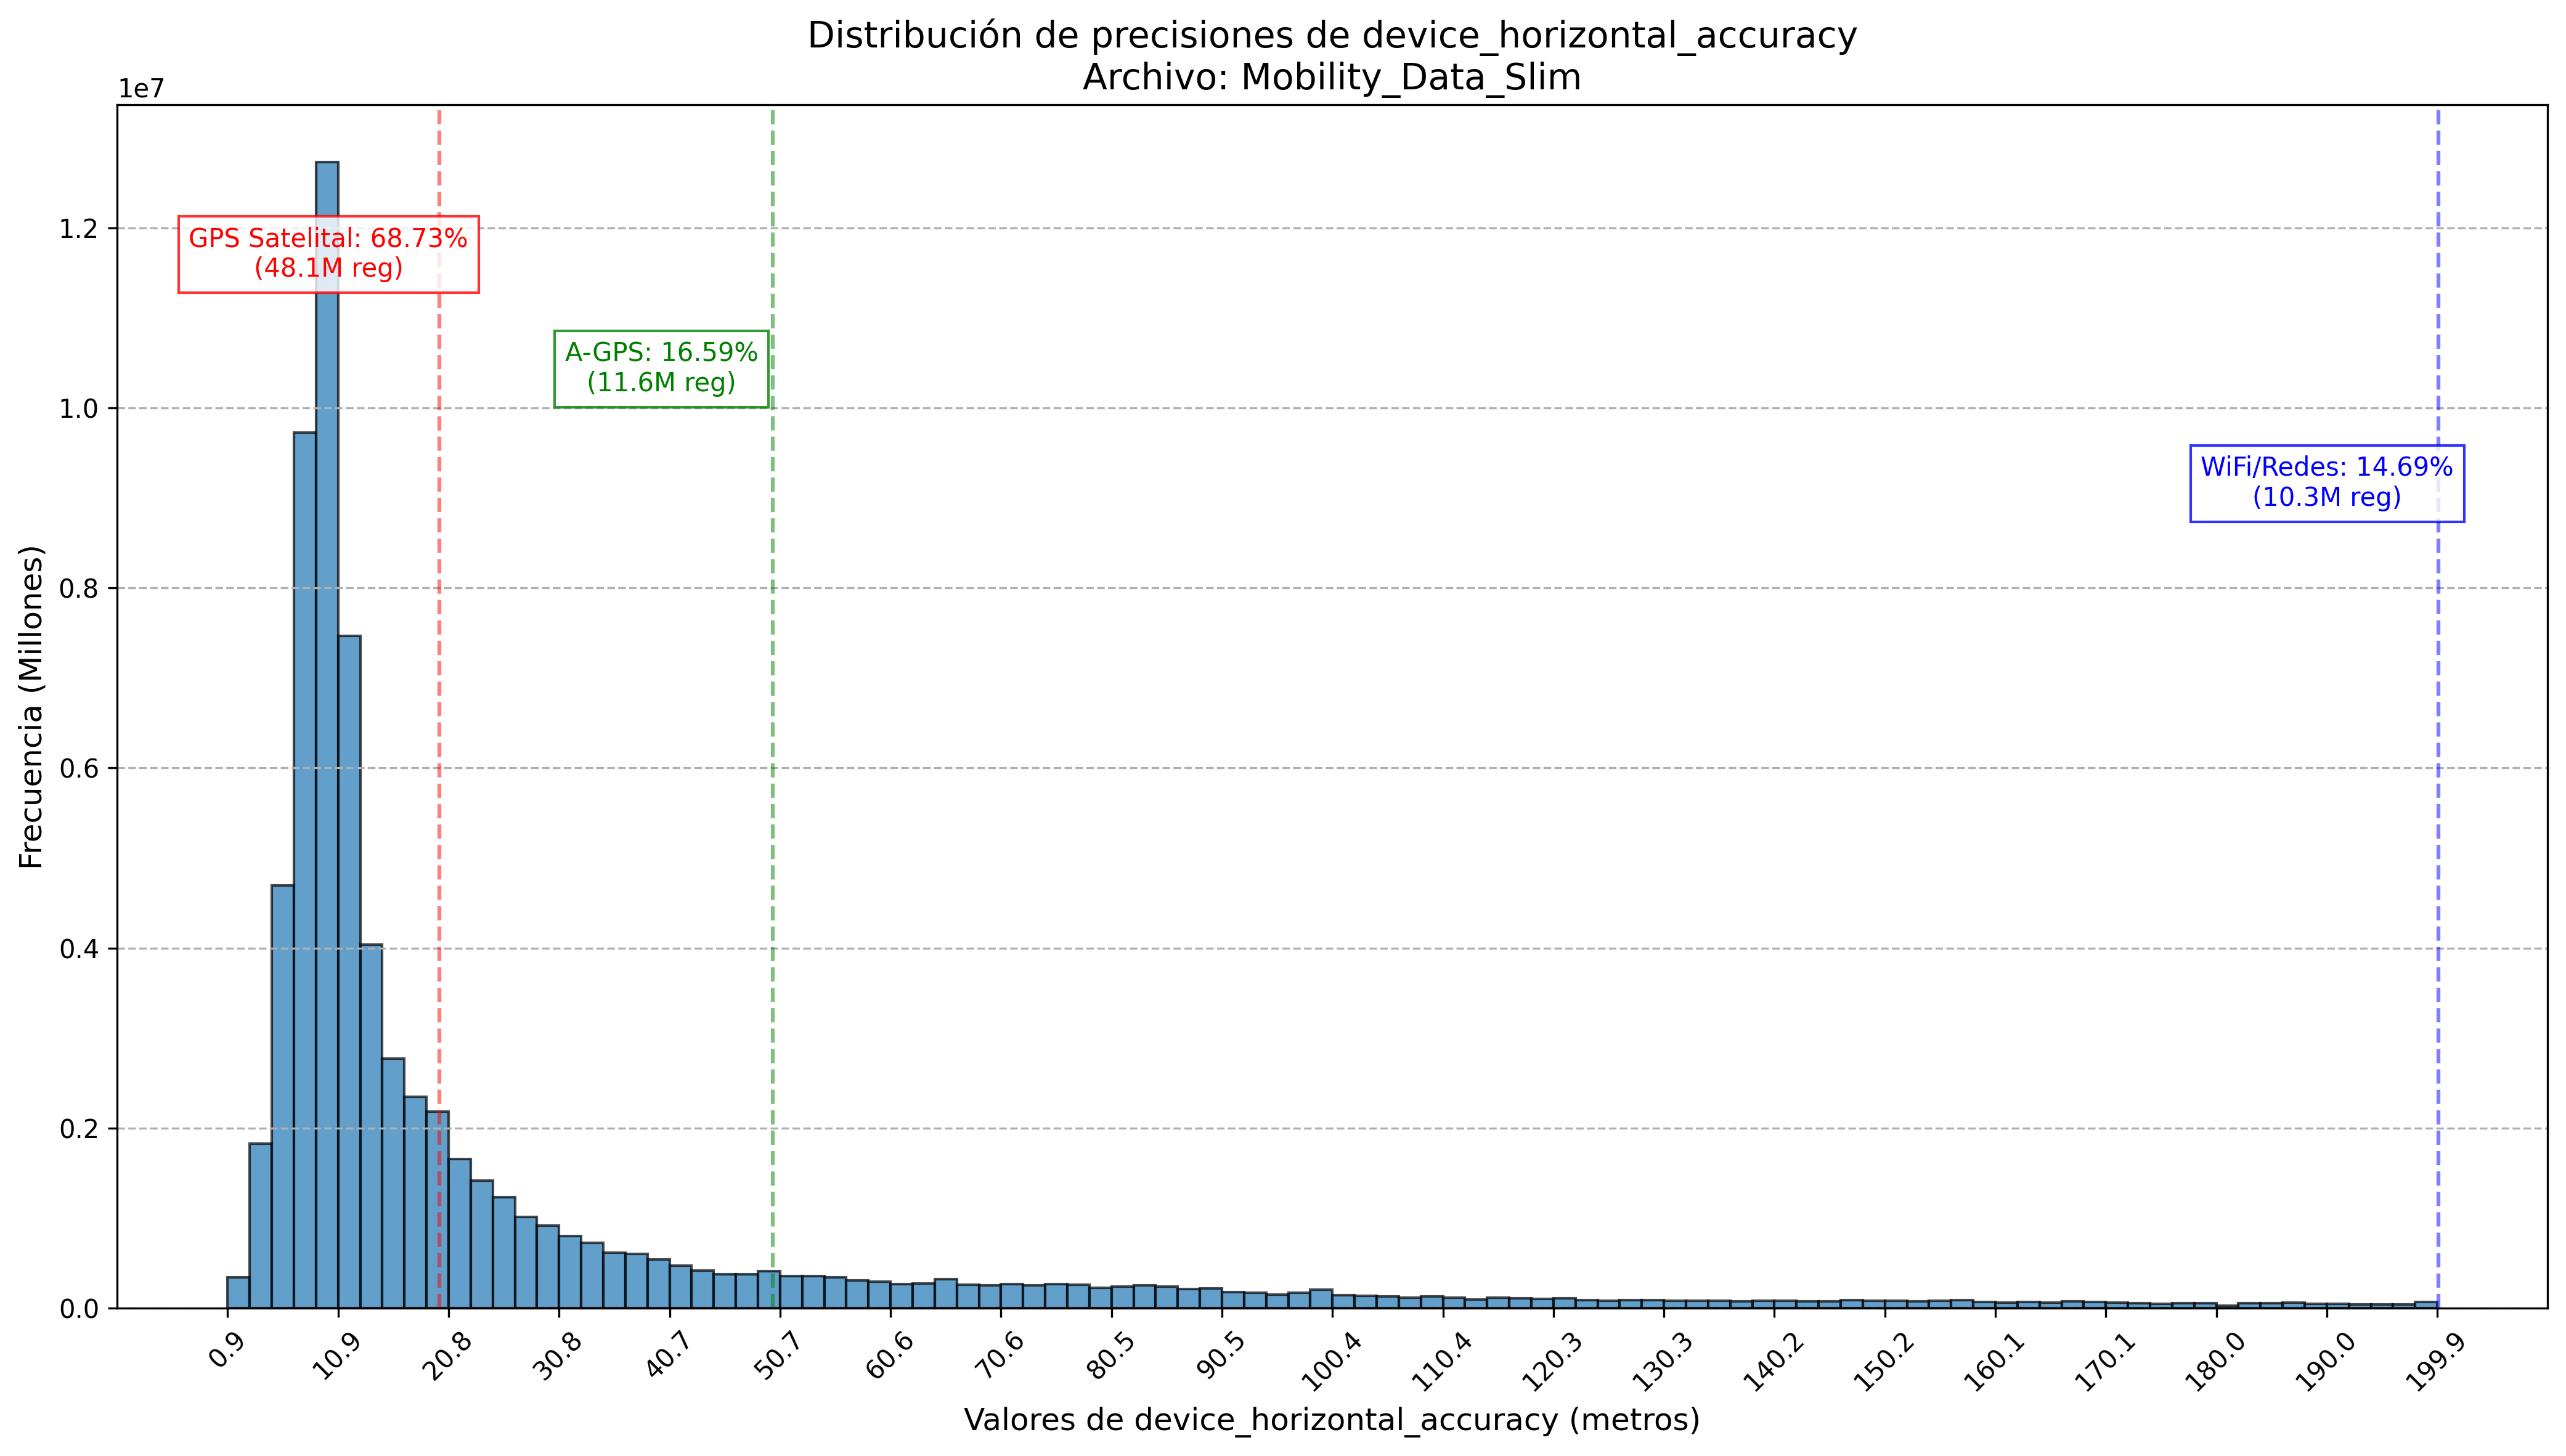
\includegraphics[width=\textwidth]{img/histograma_device_horizontal_accuracy_Mobility_Data_Slim.png}
    \caption{Frecuencia de aparación de los valores de 'device\_horizontal\_accuracy'.}
    \label{fig:accuracy_histogram}
\end{figure}

Para el objetivo de este proyecto, se busca que la configuración del GPS sea lo más precisa posible, por lo que aquellos que estén dentro del rango del GPS puro (1-20 metros) son los más relevantes. Como se puede ver en la Figura \ref{fig:accuracy_histogram}, el \textbf{68.73\%} de los valores se encuentran dentro de este rango. Sin embargo, el \textbf{31.27\%} de registros con están por encima de este rango, precisión A-GPS (5-50 metros) y triangulación por WiFi/red móvil (20-500 metros).\\
\\
La siguiente columna a evaluar es \texttt{identifier}, corresponde al identificador único de cada dispositivo.  Para analizar la frecuencia de aparición de estos valores se empleó un script que agrupa las repeticiones por rangos y grafica la cantidad de valores únicos usando escala logarítmica (ver Apéndice \ref{cod:identifier_histogram}).

\begin{figure}[H]
    \centering
    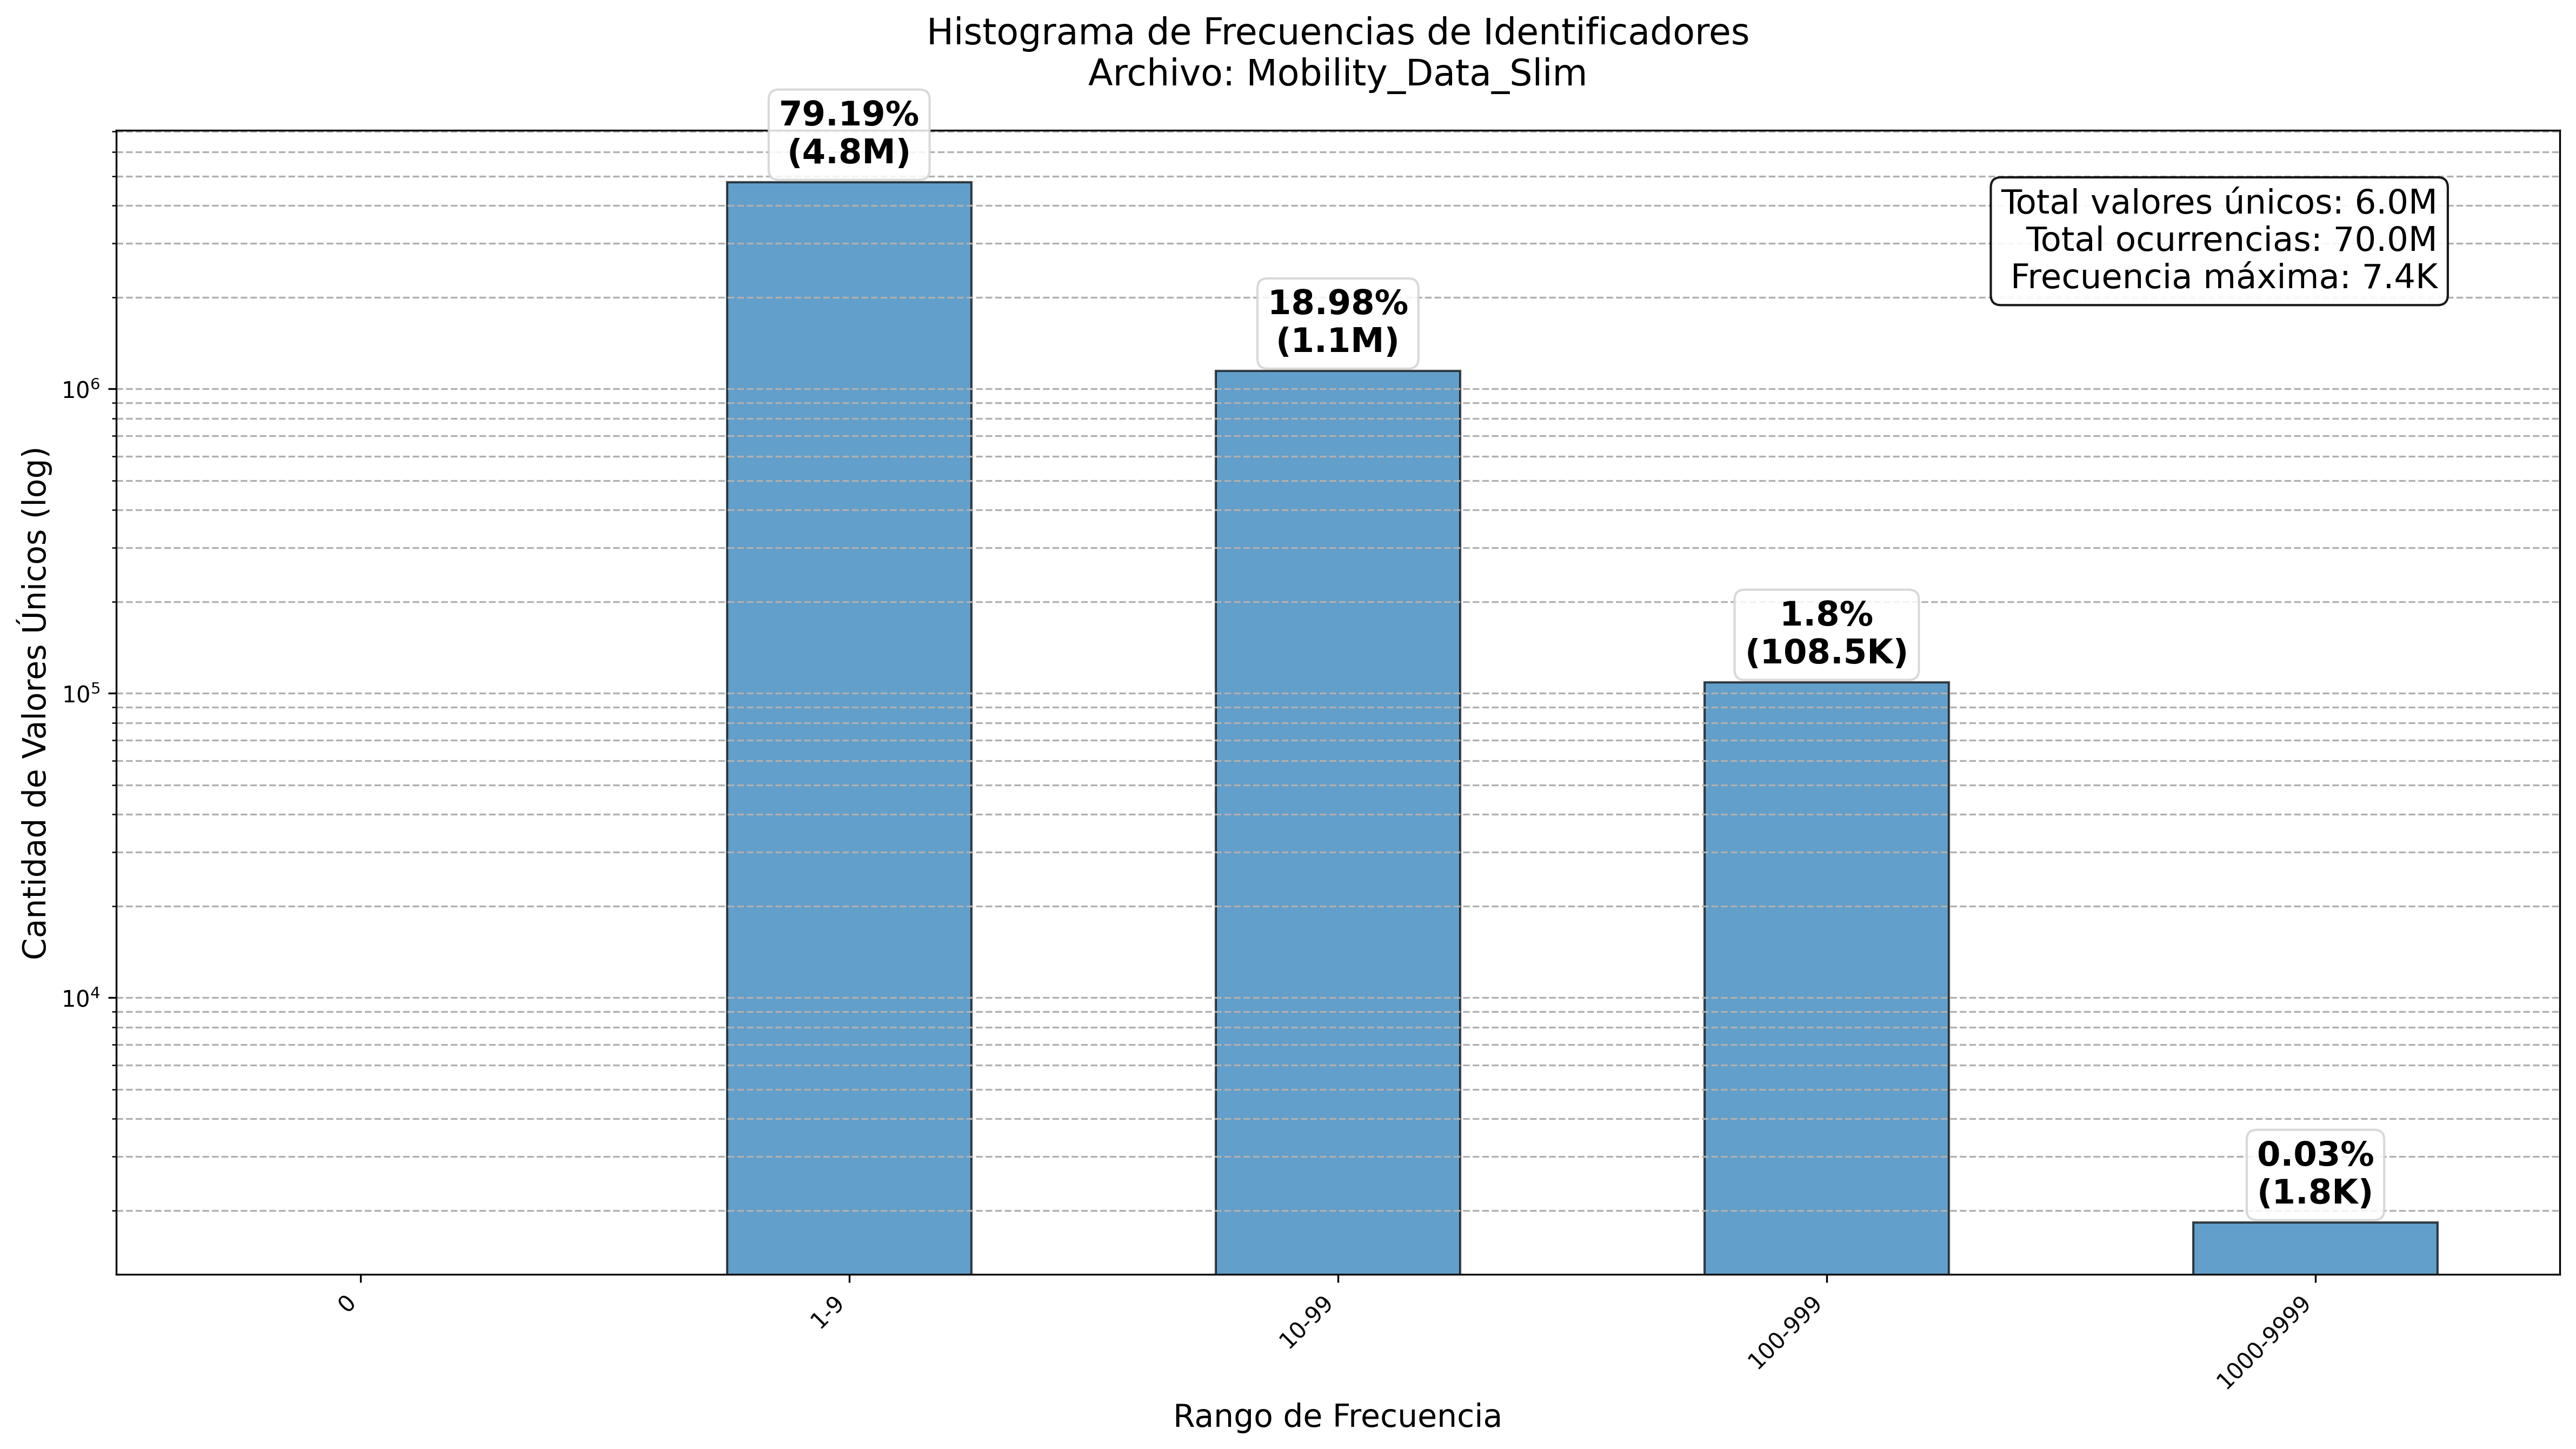
\includegraphics[width=0.8\textwidth]{img/histograma_identifier_Mobility_Data_Slim.png}
    \caption{Frecuencia de aparición de los identificadores únicos.}
    \label{fig:identifier_histogram}
\end{figure}

 De este script sabemos que el total de individuos es de \textbf{6,022,772} de los cuales el \textbf{79.19\%} tienen una frecuencia de aparición de una a nueve veces, esto es \textbf{4,769,317} de individuos. Así mismo de la Figura \ref{fig:identifier_histogram} podemos observar que hay poco más de un \textbf{20\%} de individuos con más de 99 repeticiones. Por lo que se necesita hacer un análisis más detallado, para ello se ejecuta el código del Apéndice \ref{cod:identifier_histogram_detailed}, el cual segmenta los datos en tres rangos: 1-99, 100-1000 y 1001-10000 repeticiones.

\begin{figure}[htbp]
    \centering
    \begin{subfigure}[t]{0.48\textwidth-1em}
        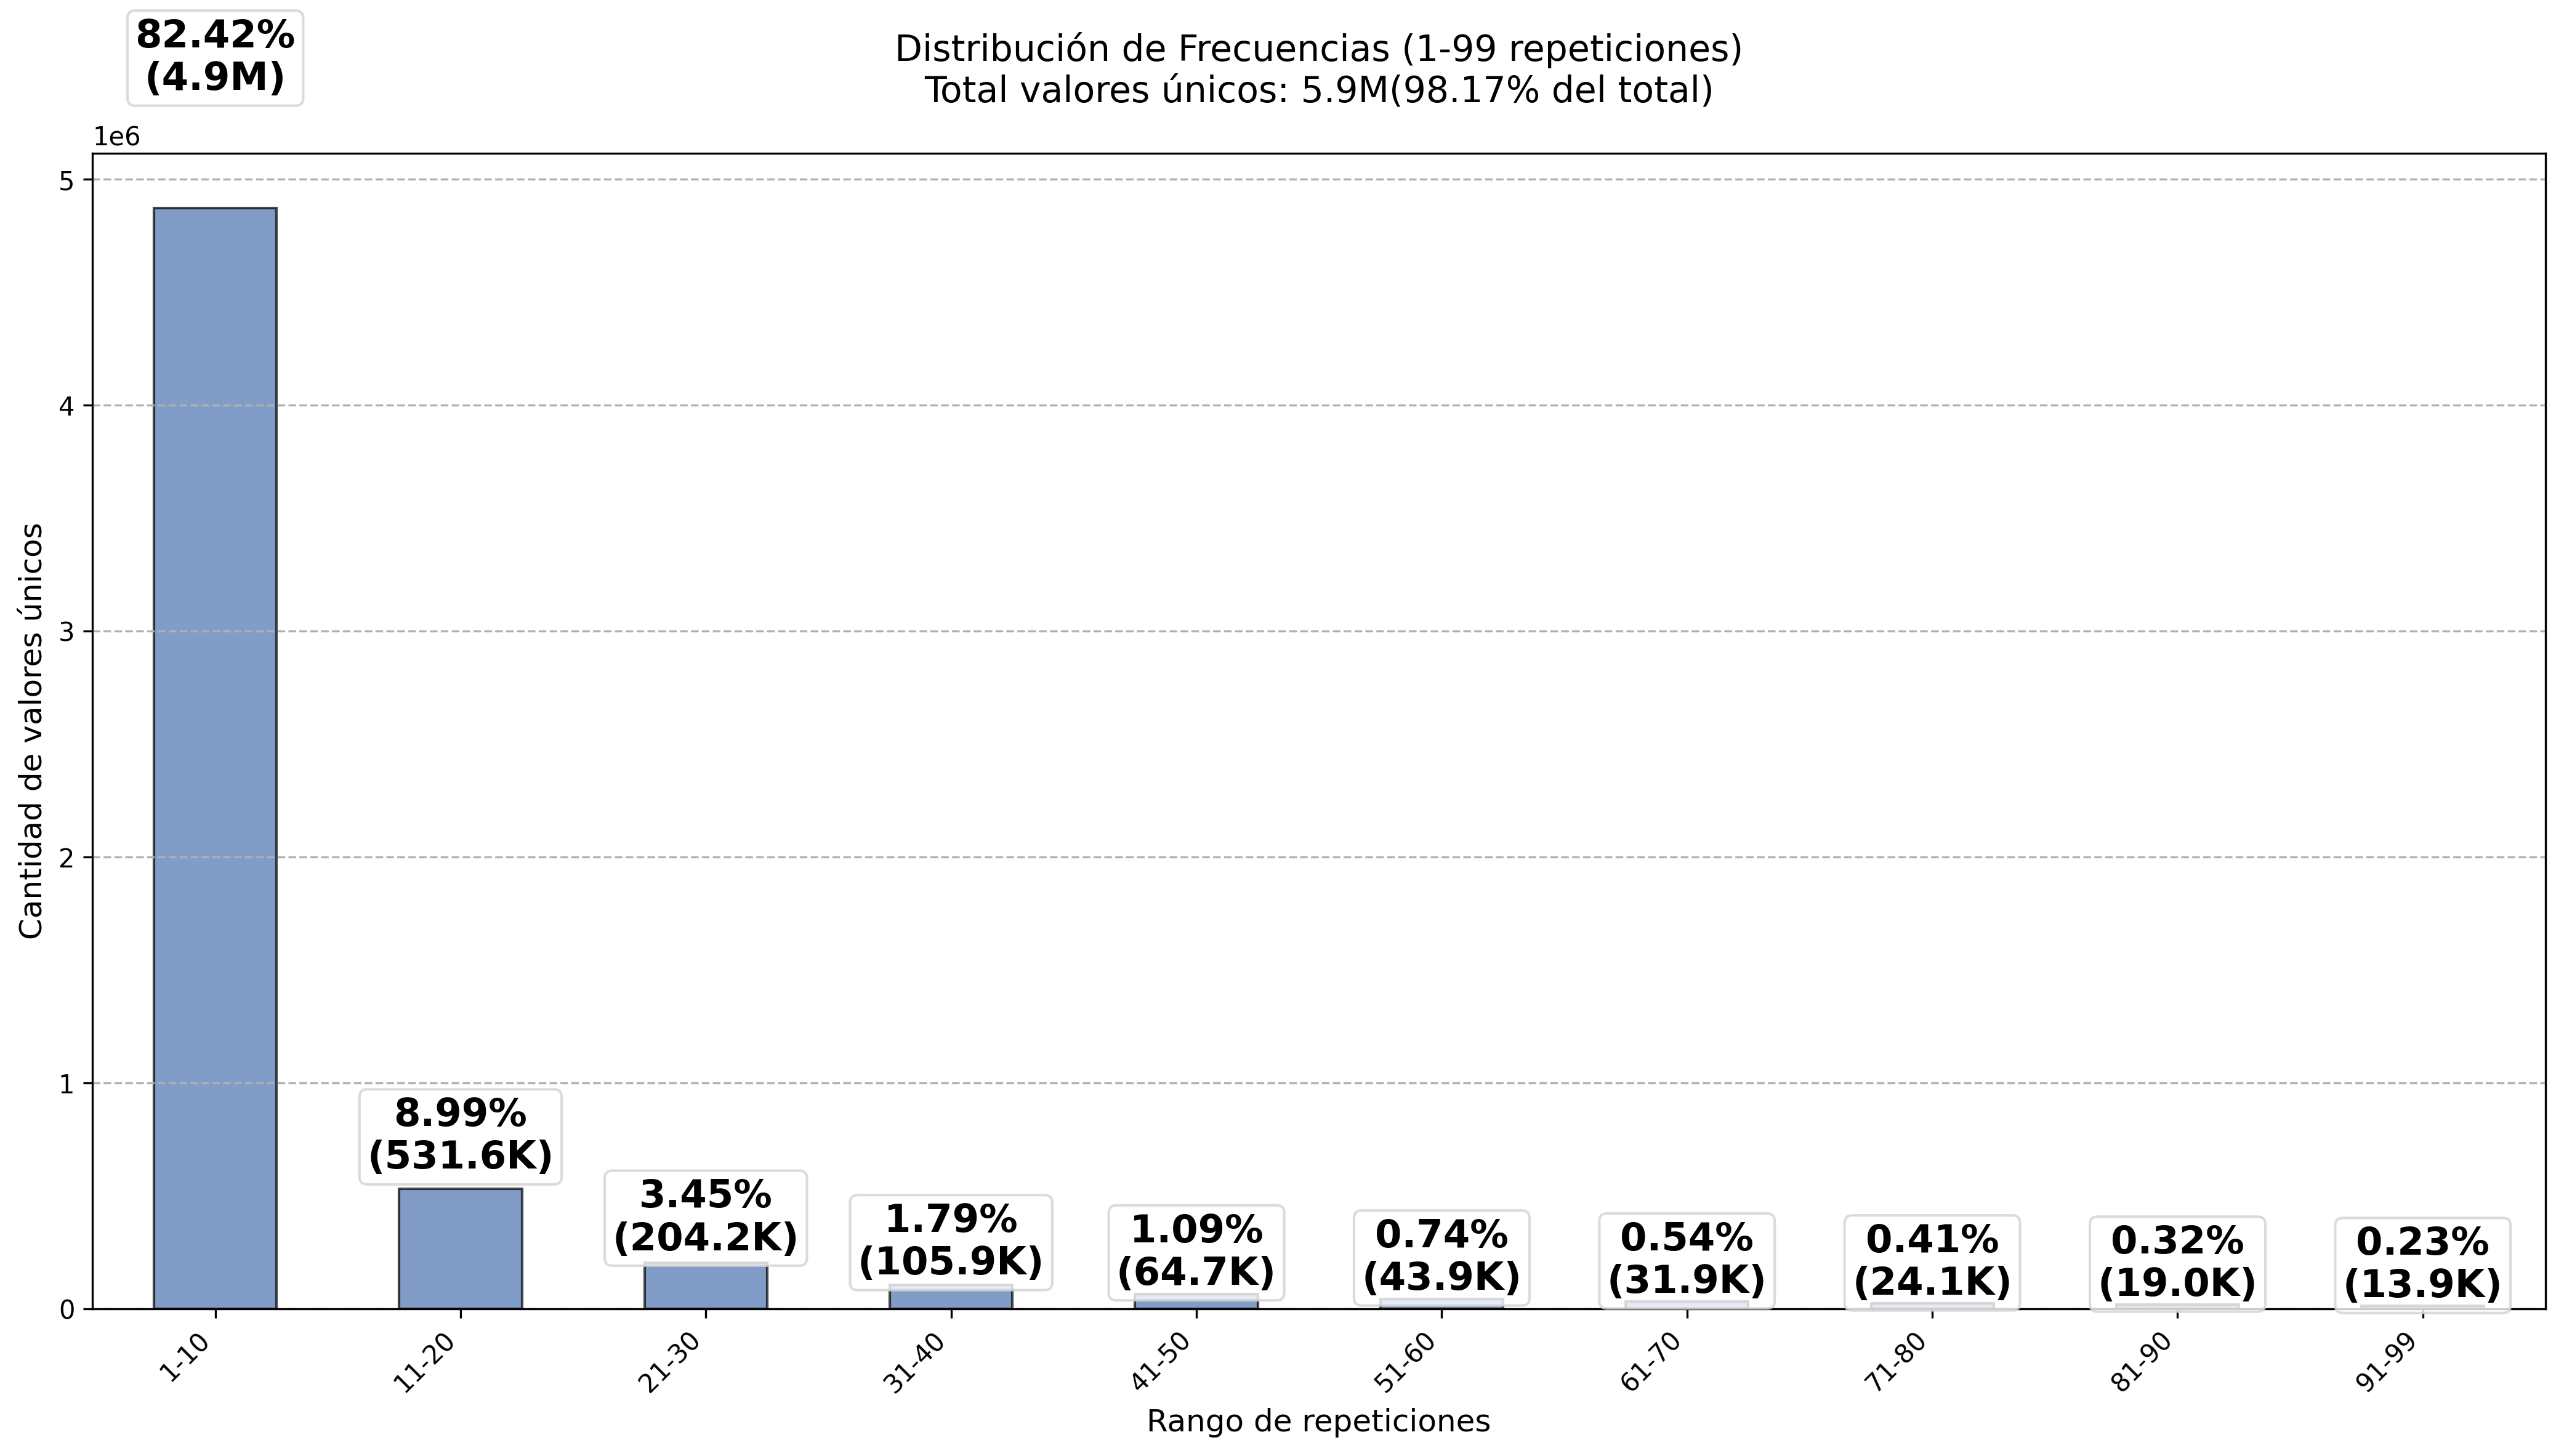
\includegraphics[width=\linewidth]{img/histograma_1-99_identifier_Mobility_Data_Slim.png}
        \caption{Histograma 1-99 repeticiones}
        \label{fig:sub1}
    \end{subfigure}
    \hfill
    \begin{subfigure}[t]{0.48\textwidth-1em}
        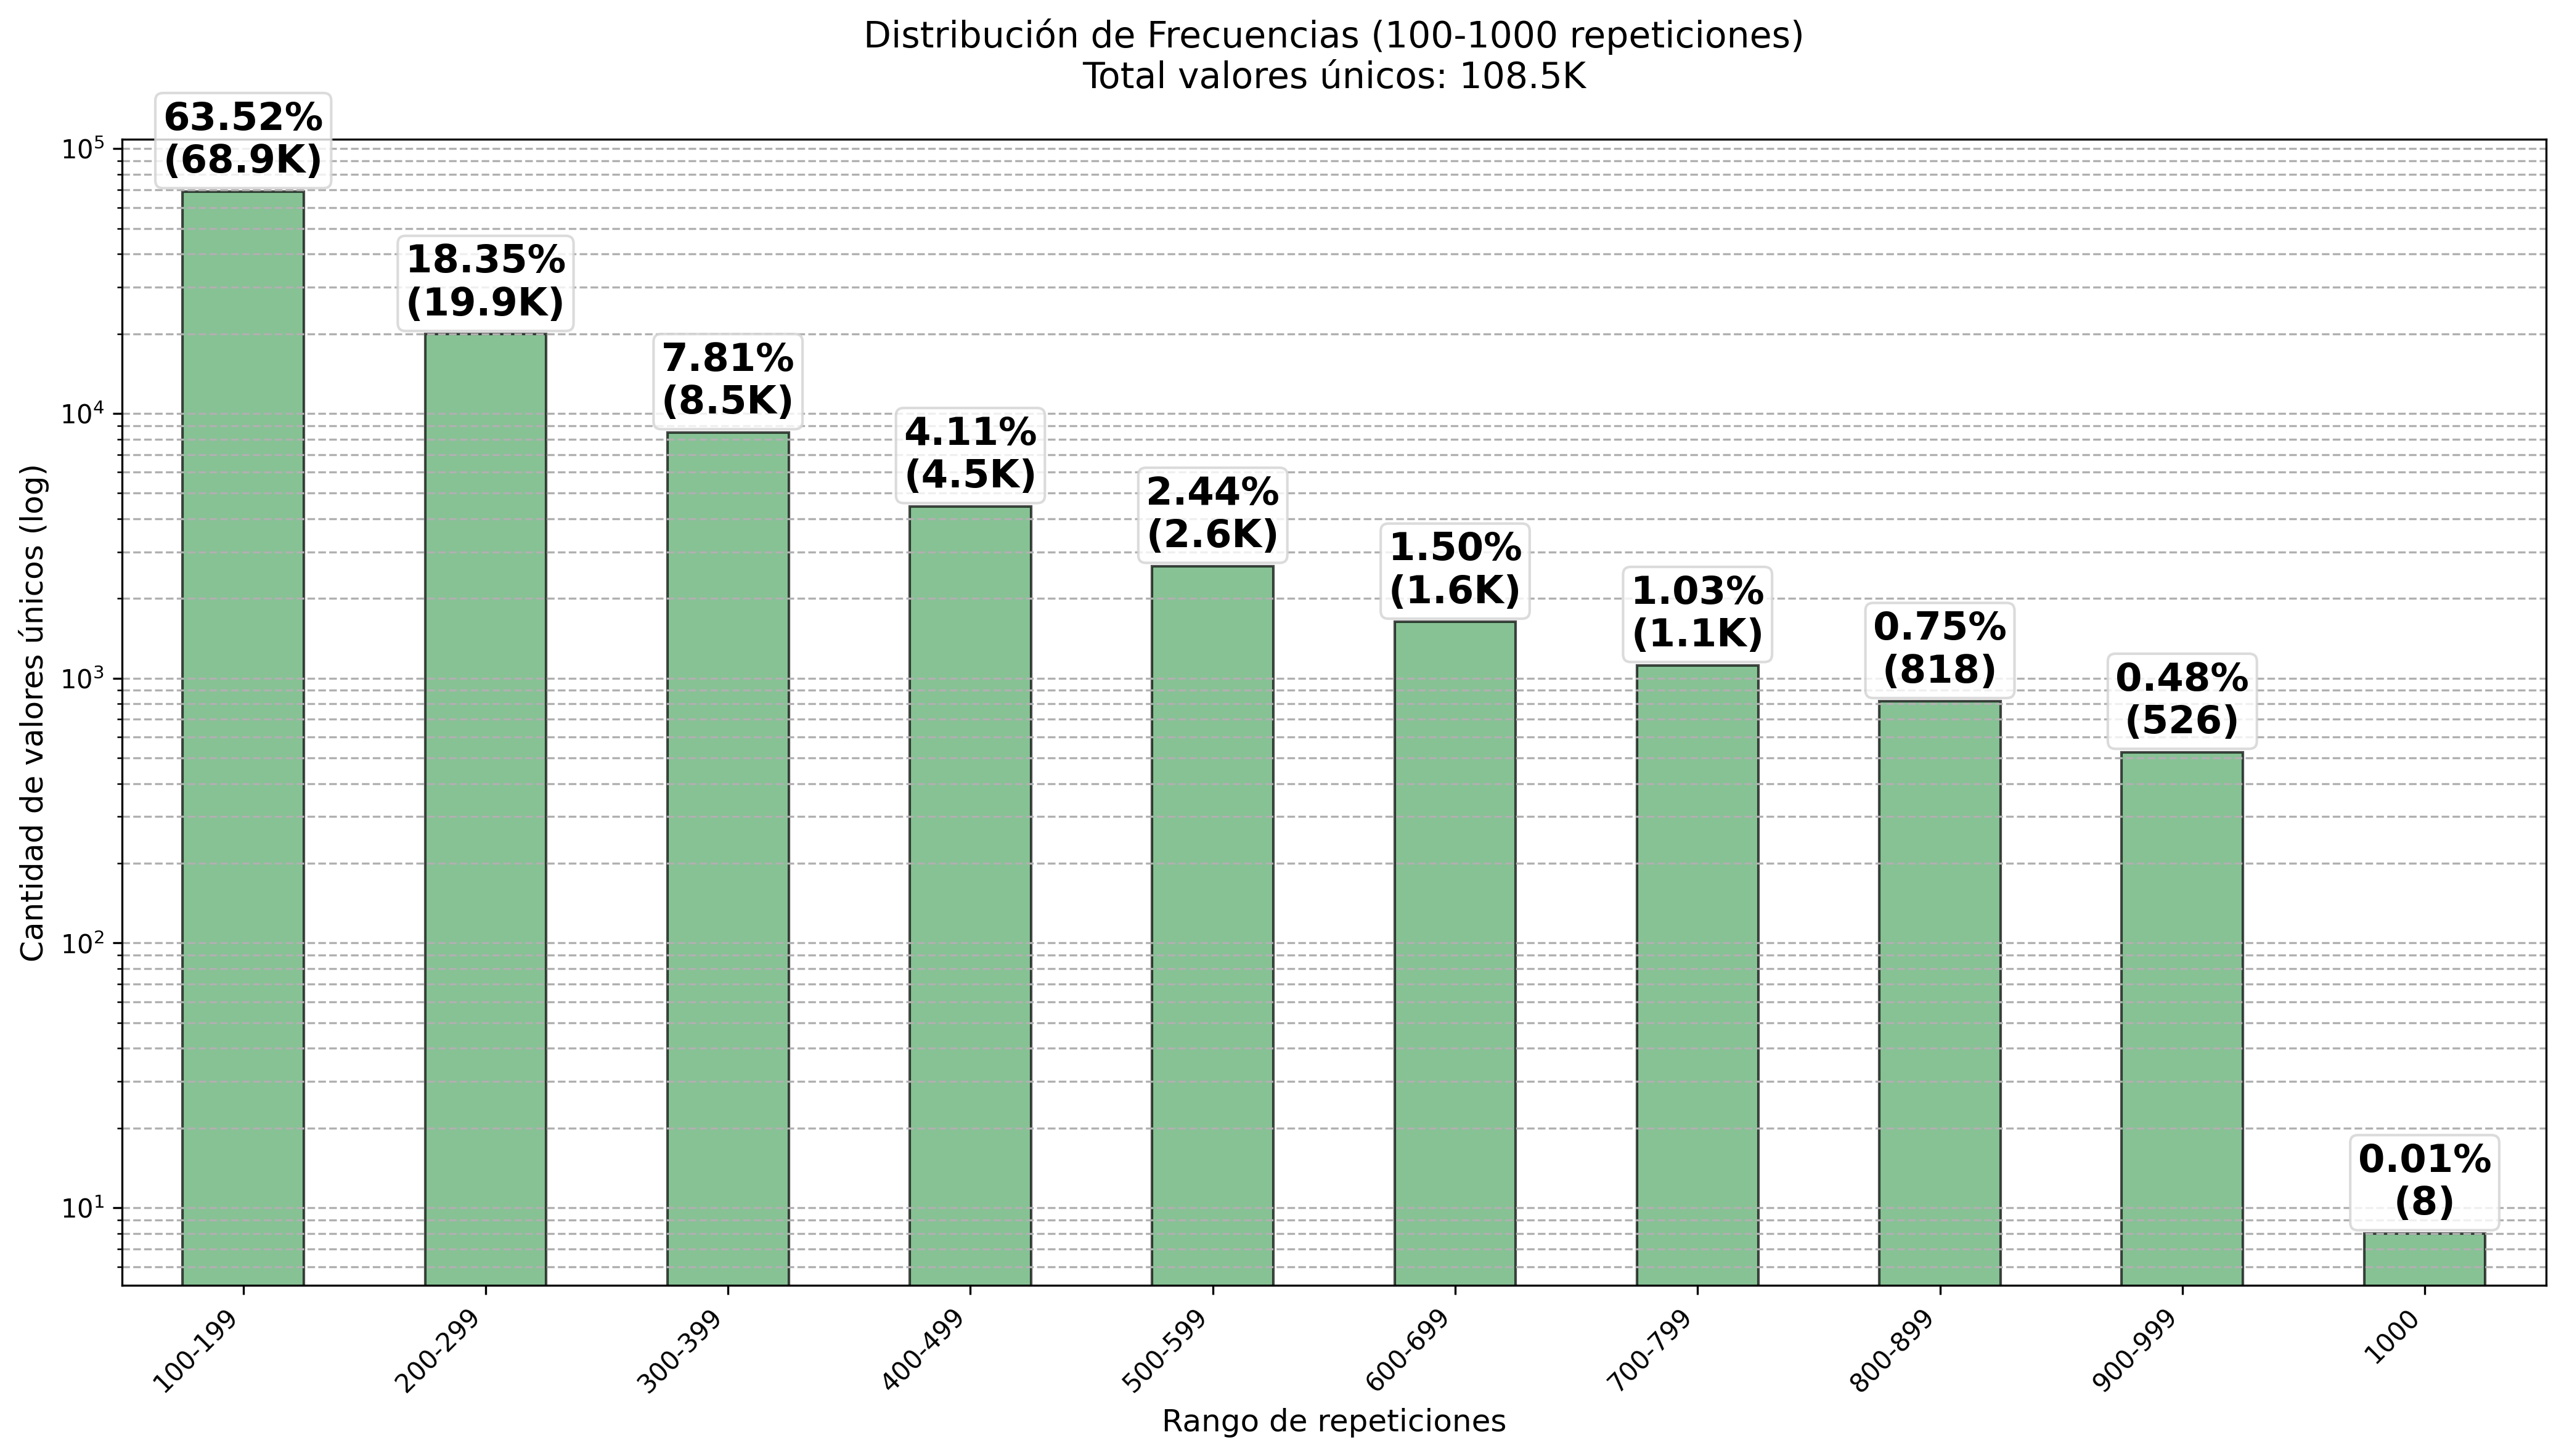
\includegraphics[width=\linewidth]{img/histograma_100-1k_identifier_Mobility_Data_Slim.png}
        \caption{Histograma 100–1000 repeticiones}
        \label{fig:sub2}
    \end{subfigure}

    \vspace{0.5cm}

    \begin{subfigure}[t]{0.48\textwidth}
        \centering
        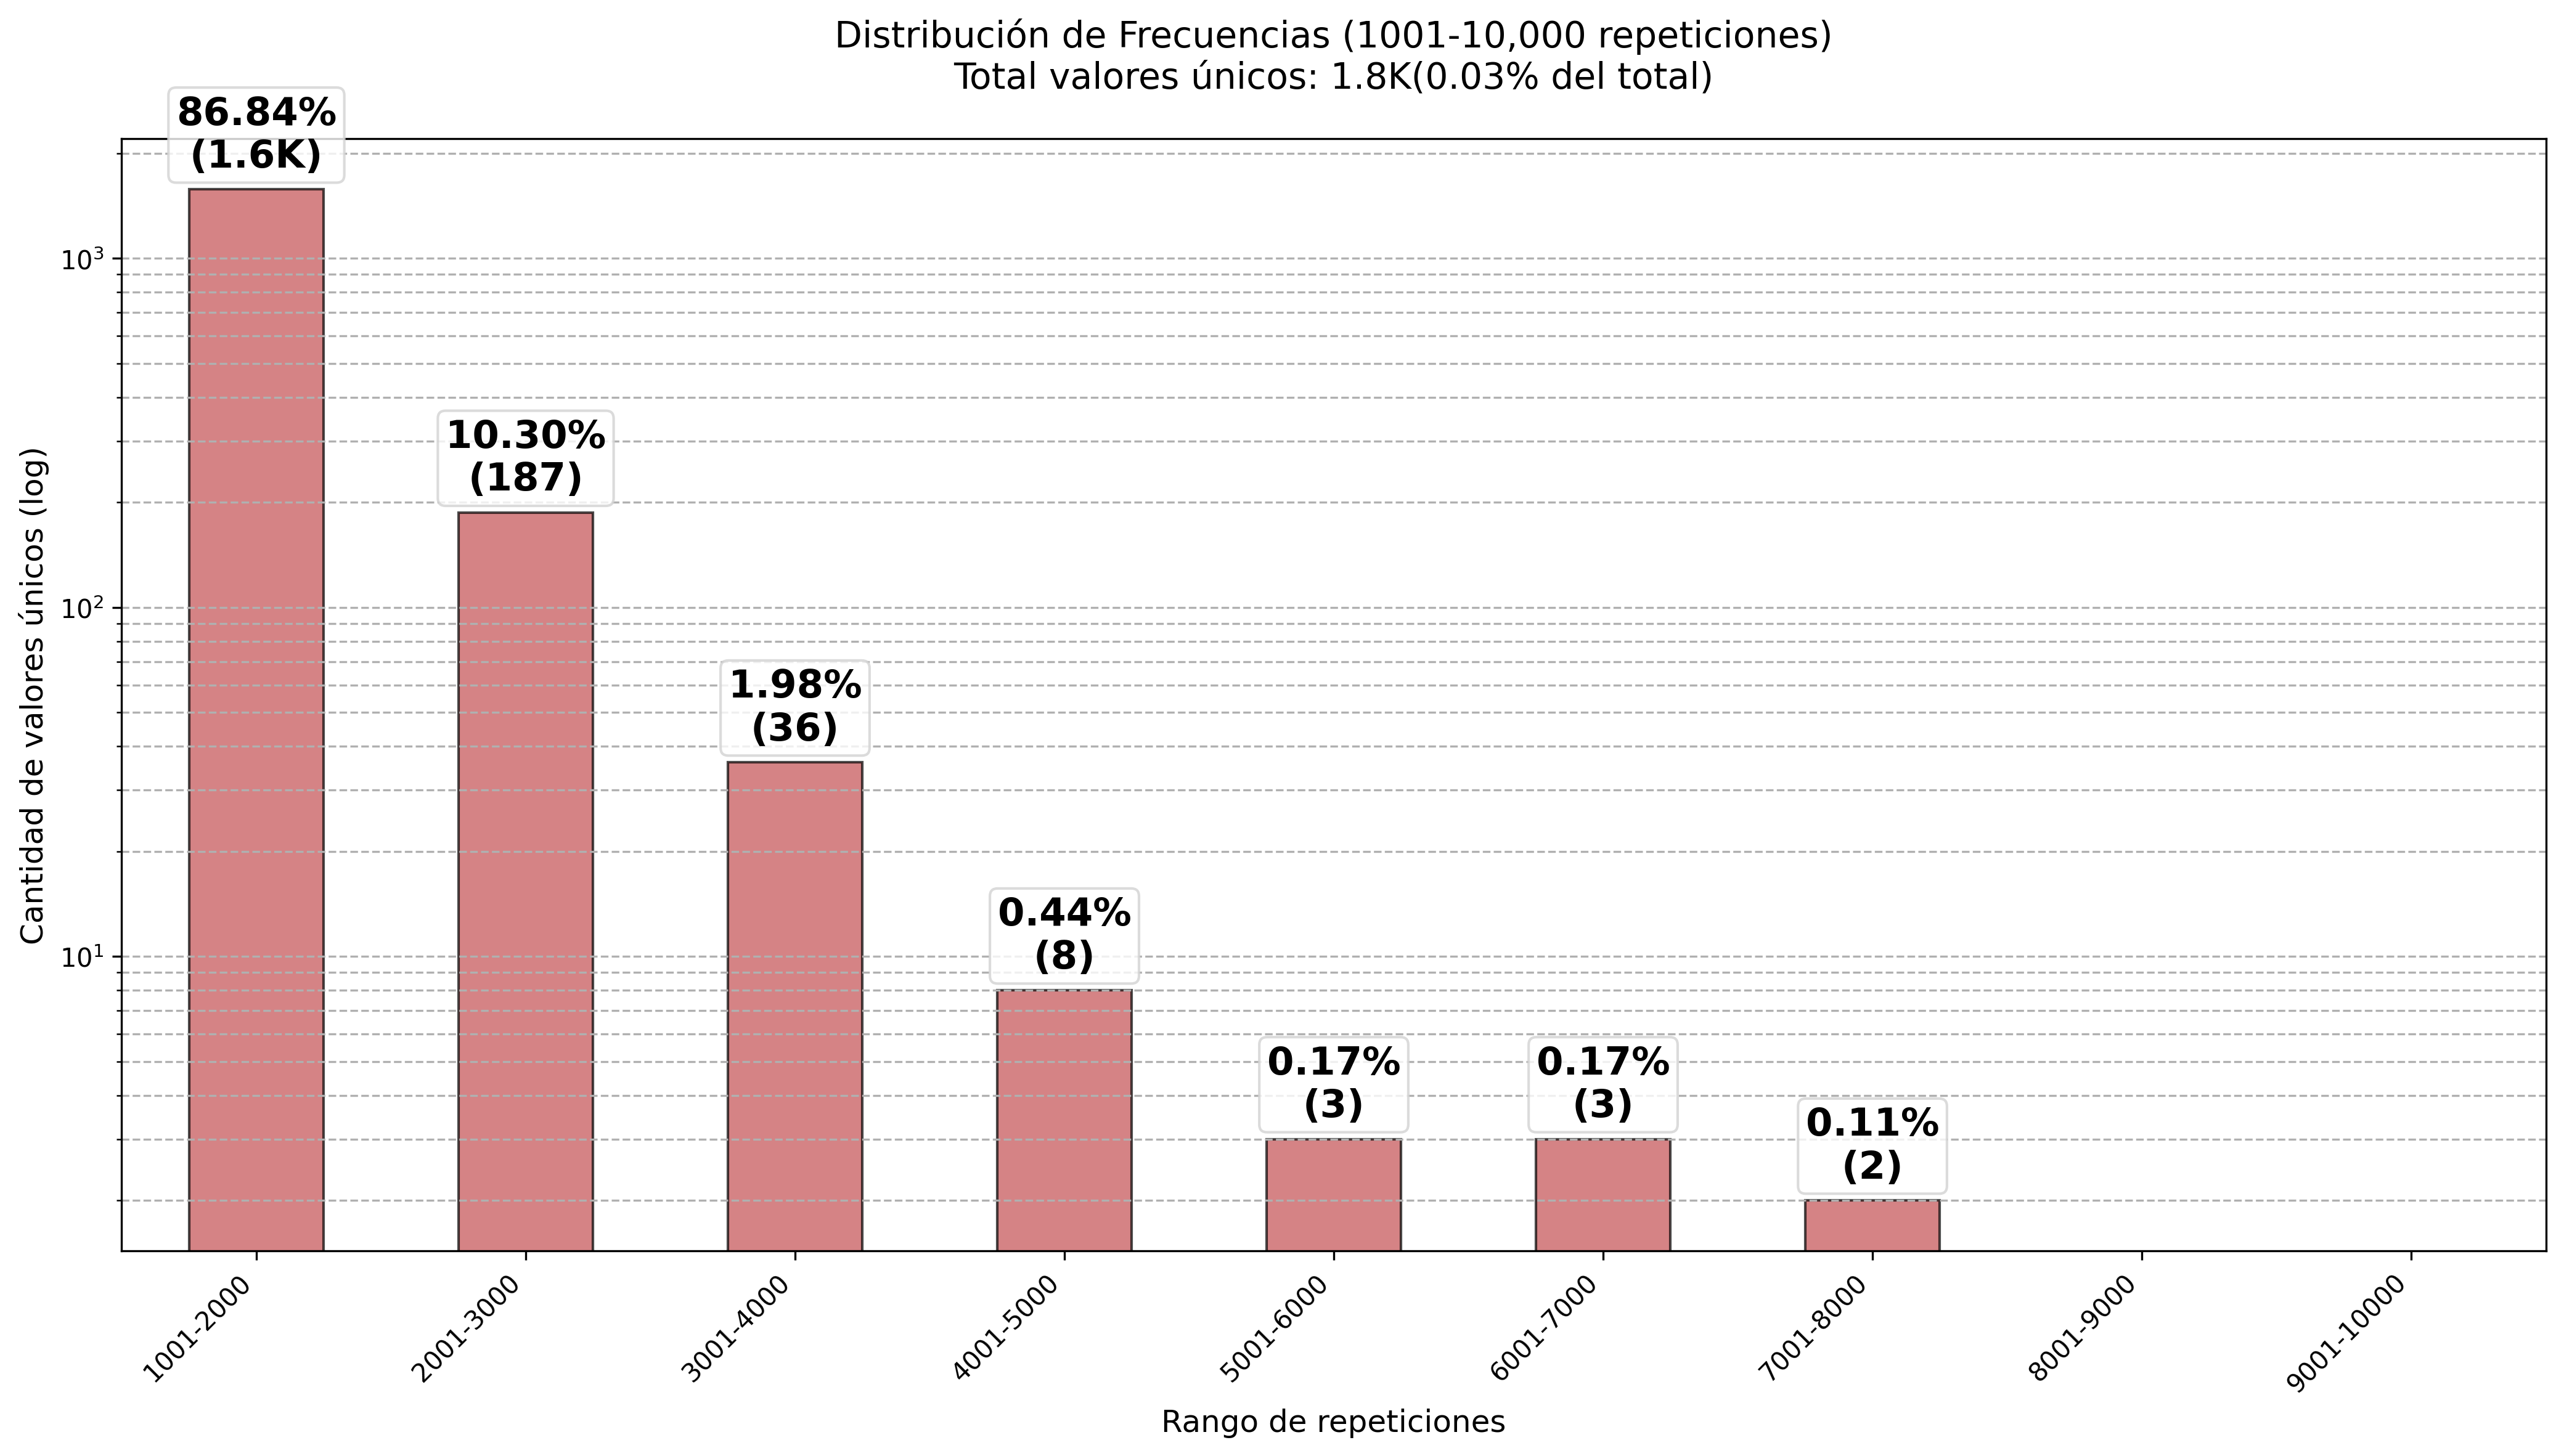
\includegraphics[width=\linewidth]{img/histograma_1k-10k_identifier_Mobility_Data_Slim.png}
        \caption{Histograma 1001–10000 repeticiones}
        \label{fig:sub3}
    \end{subfigure}

    \caption{Comparación de histogramas por rangos de repeticiones.}
    \label{fig:histogramas}
\end{figure}

Con la información obtenida de los histogramas de la figura anterior, se puede observar que el \textbf{98.17\%} de los identificadores únicos tienen entre 1 y 99 repeticiones, lo que equivale a \textbf{5,912,437} individuos. Por otro lado, el \textbf{1.83\%} restante tiene entre 100 y 10,000 repeticiones, lo que equivale a \textbf{110,335} individuos. Con base en esta información aún no se puede determinar que registros eliminar. Por lo que ahora se eliminarán aquellos registros que sean duplicados, es decir, aquellos que tengan el mismo 
\texttt{identifier}, \texttt{timestamp}, \texttt{device\_lat} y \texttt{device\_lon}. Para ello se utilizó el código del Apéndice \ref{cod:csv_deduplicate}, que elimina los duplicados y genera un nuevo archivo CSV con los registros de individuos. \\
Con este nuevo archivo se vuelve a realizar el análisis de frecuencia de aparición de individuos. En la siguiente figura se muestra el histograma de la frecuencia de aparición de los identificadores únicos

\begin{figure}[H]
    \centering
    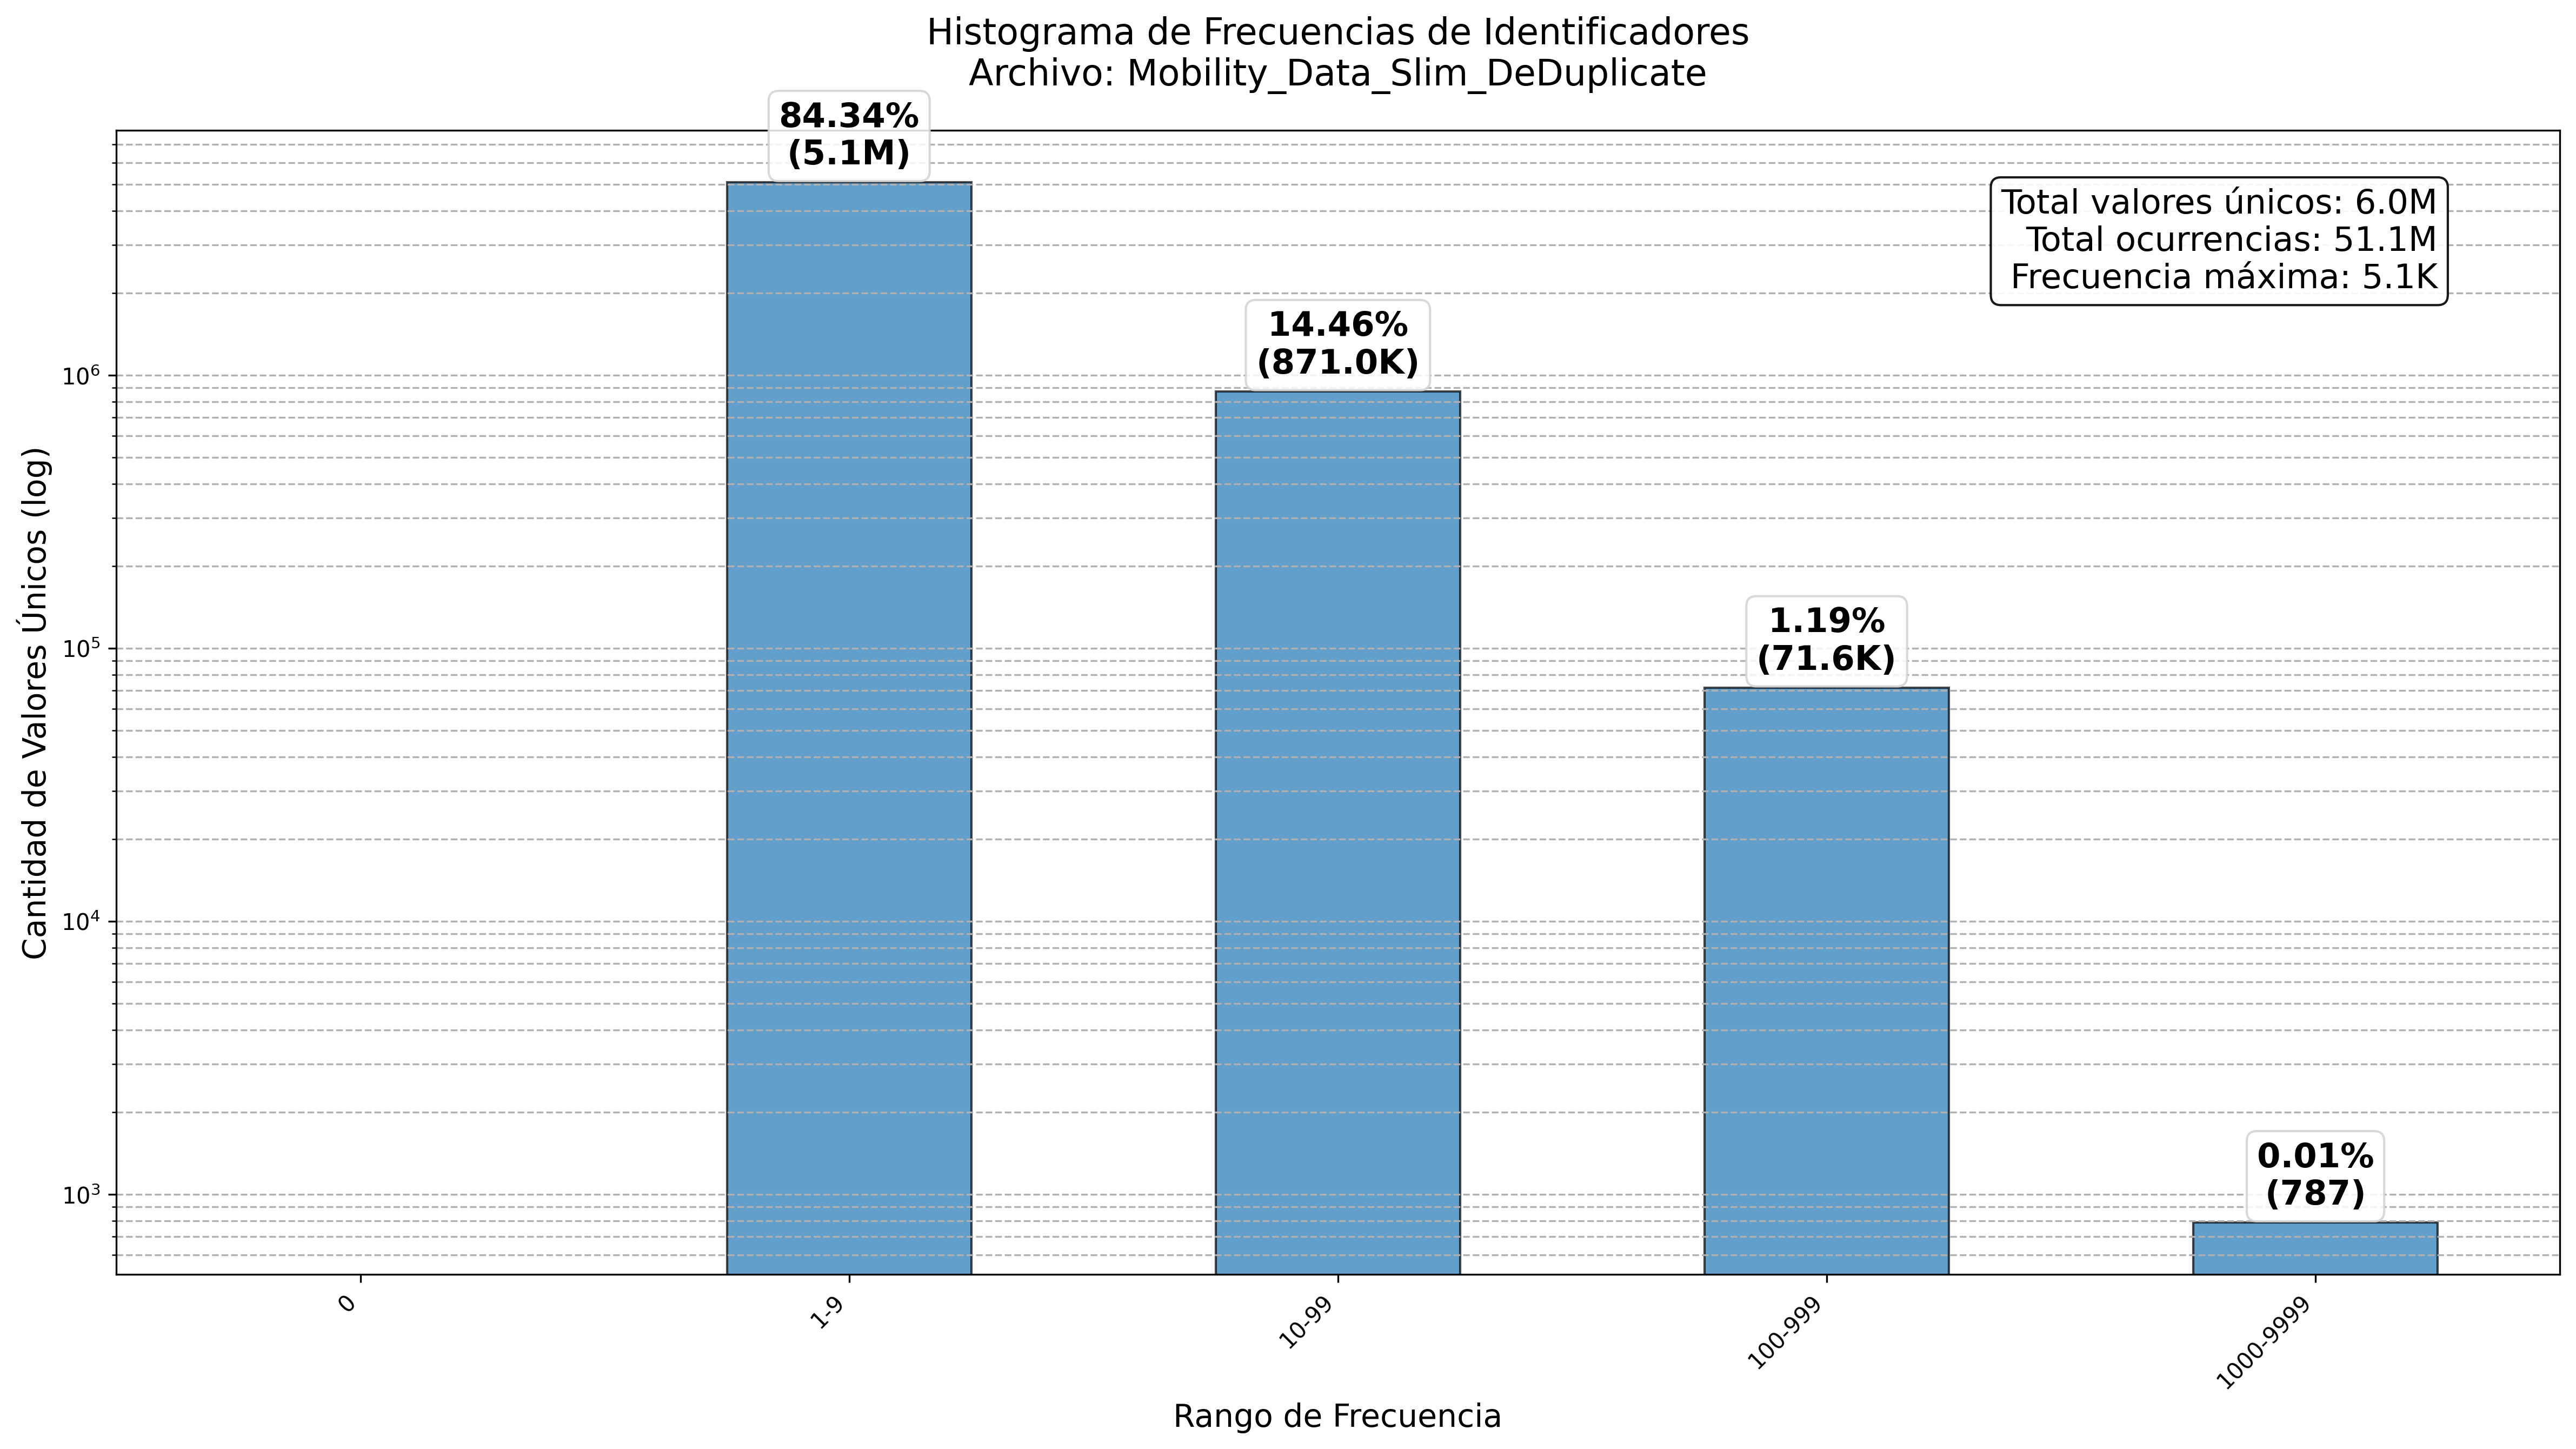
\includegraphics[width=0.8\textwidth]{img/histograma_identifier_Mobility_Data_Slim_DeDuplicate.png}
    \caption{Frecuencia de aparición de los identificadores únicos después de eliminar duplicados.}
    \label{fig:identifier_histogram_deduplicate}
\end{figure}

Comparando los resultados de la Figura \ref{fig:identifier_histogram} y la Figura \ref{fig:identifier_histogram_deduplicate} podemos destacar varios hallazgos importantes: 

\begin{description}
    \item[Preservación de la diversidad de individuos]: Los \textbf{6,022,772} únicos se mantuvieron sin cambios.
    \item[Reducción de redundancias]: La eliminación del \textbf{27\%} de registros. De \textbf{70 millones} a \textbf{51 millones} de registros.
    \item[Correcció de sesgos]: La reducción del \textbf{31.1\%} en la frecuencia máxima de aparición (de 7,400 a 5,100) corrige sesgos que afectaban especialmente a individuos con alta frecuencia de registros repetidos. 
\end{description}

Como podemos ver la Figura \ref{fig:histogramasDeDuplicate} la distribución de los individuos se mantiene similar; sin embargo, el \textbf{98.8\%} de los identificadores únicos tienen entre 1 y 99 repeticiones, lo que equivale a \textbf{5,950,336} individuos. Por otro lado, el \textbf{1.2\%} restante tiene entre 100 y 10,000 repeticiones, lo que equivale a \textbf{72,436} individuos. Con estos datos podemos concluir que la mayoría de los individuos tienen un número limitado de registros, lo que sugiere que la mayoría de los usuarios no están generando datos de manera continua o frecuente. 
Ahora bien para poder tener una mejor idea de la distribución de los individuos, se analiza la distribución de los individuos sin duplicados para cada día registrado en el conjunto de datos. Para ello se utilizó el código del Apéndice \ref{cod:identifier_histogram_daily}.

\begin{figure}[H]
    \centering
    \begin{subfigure}[t]{0.48\textwidth-1em}
        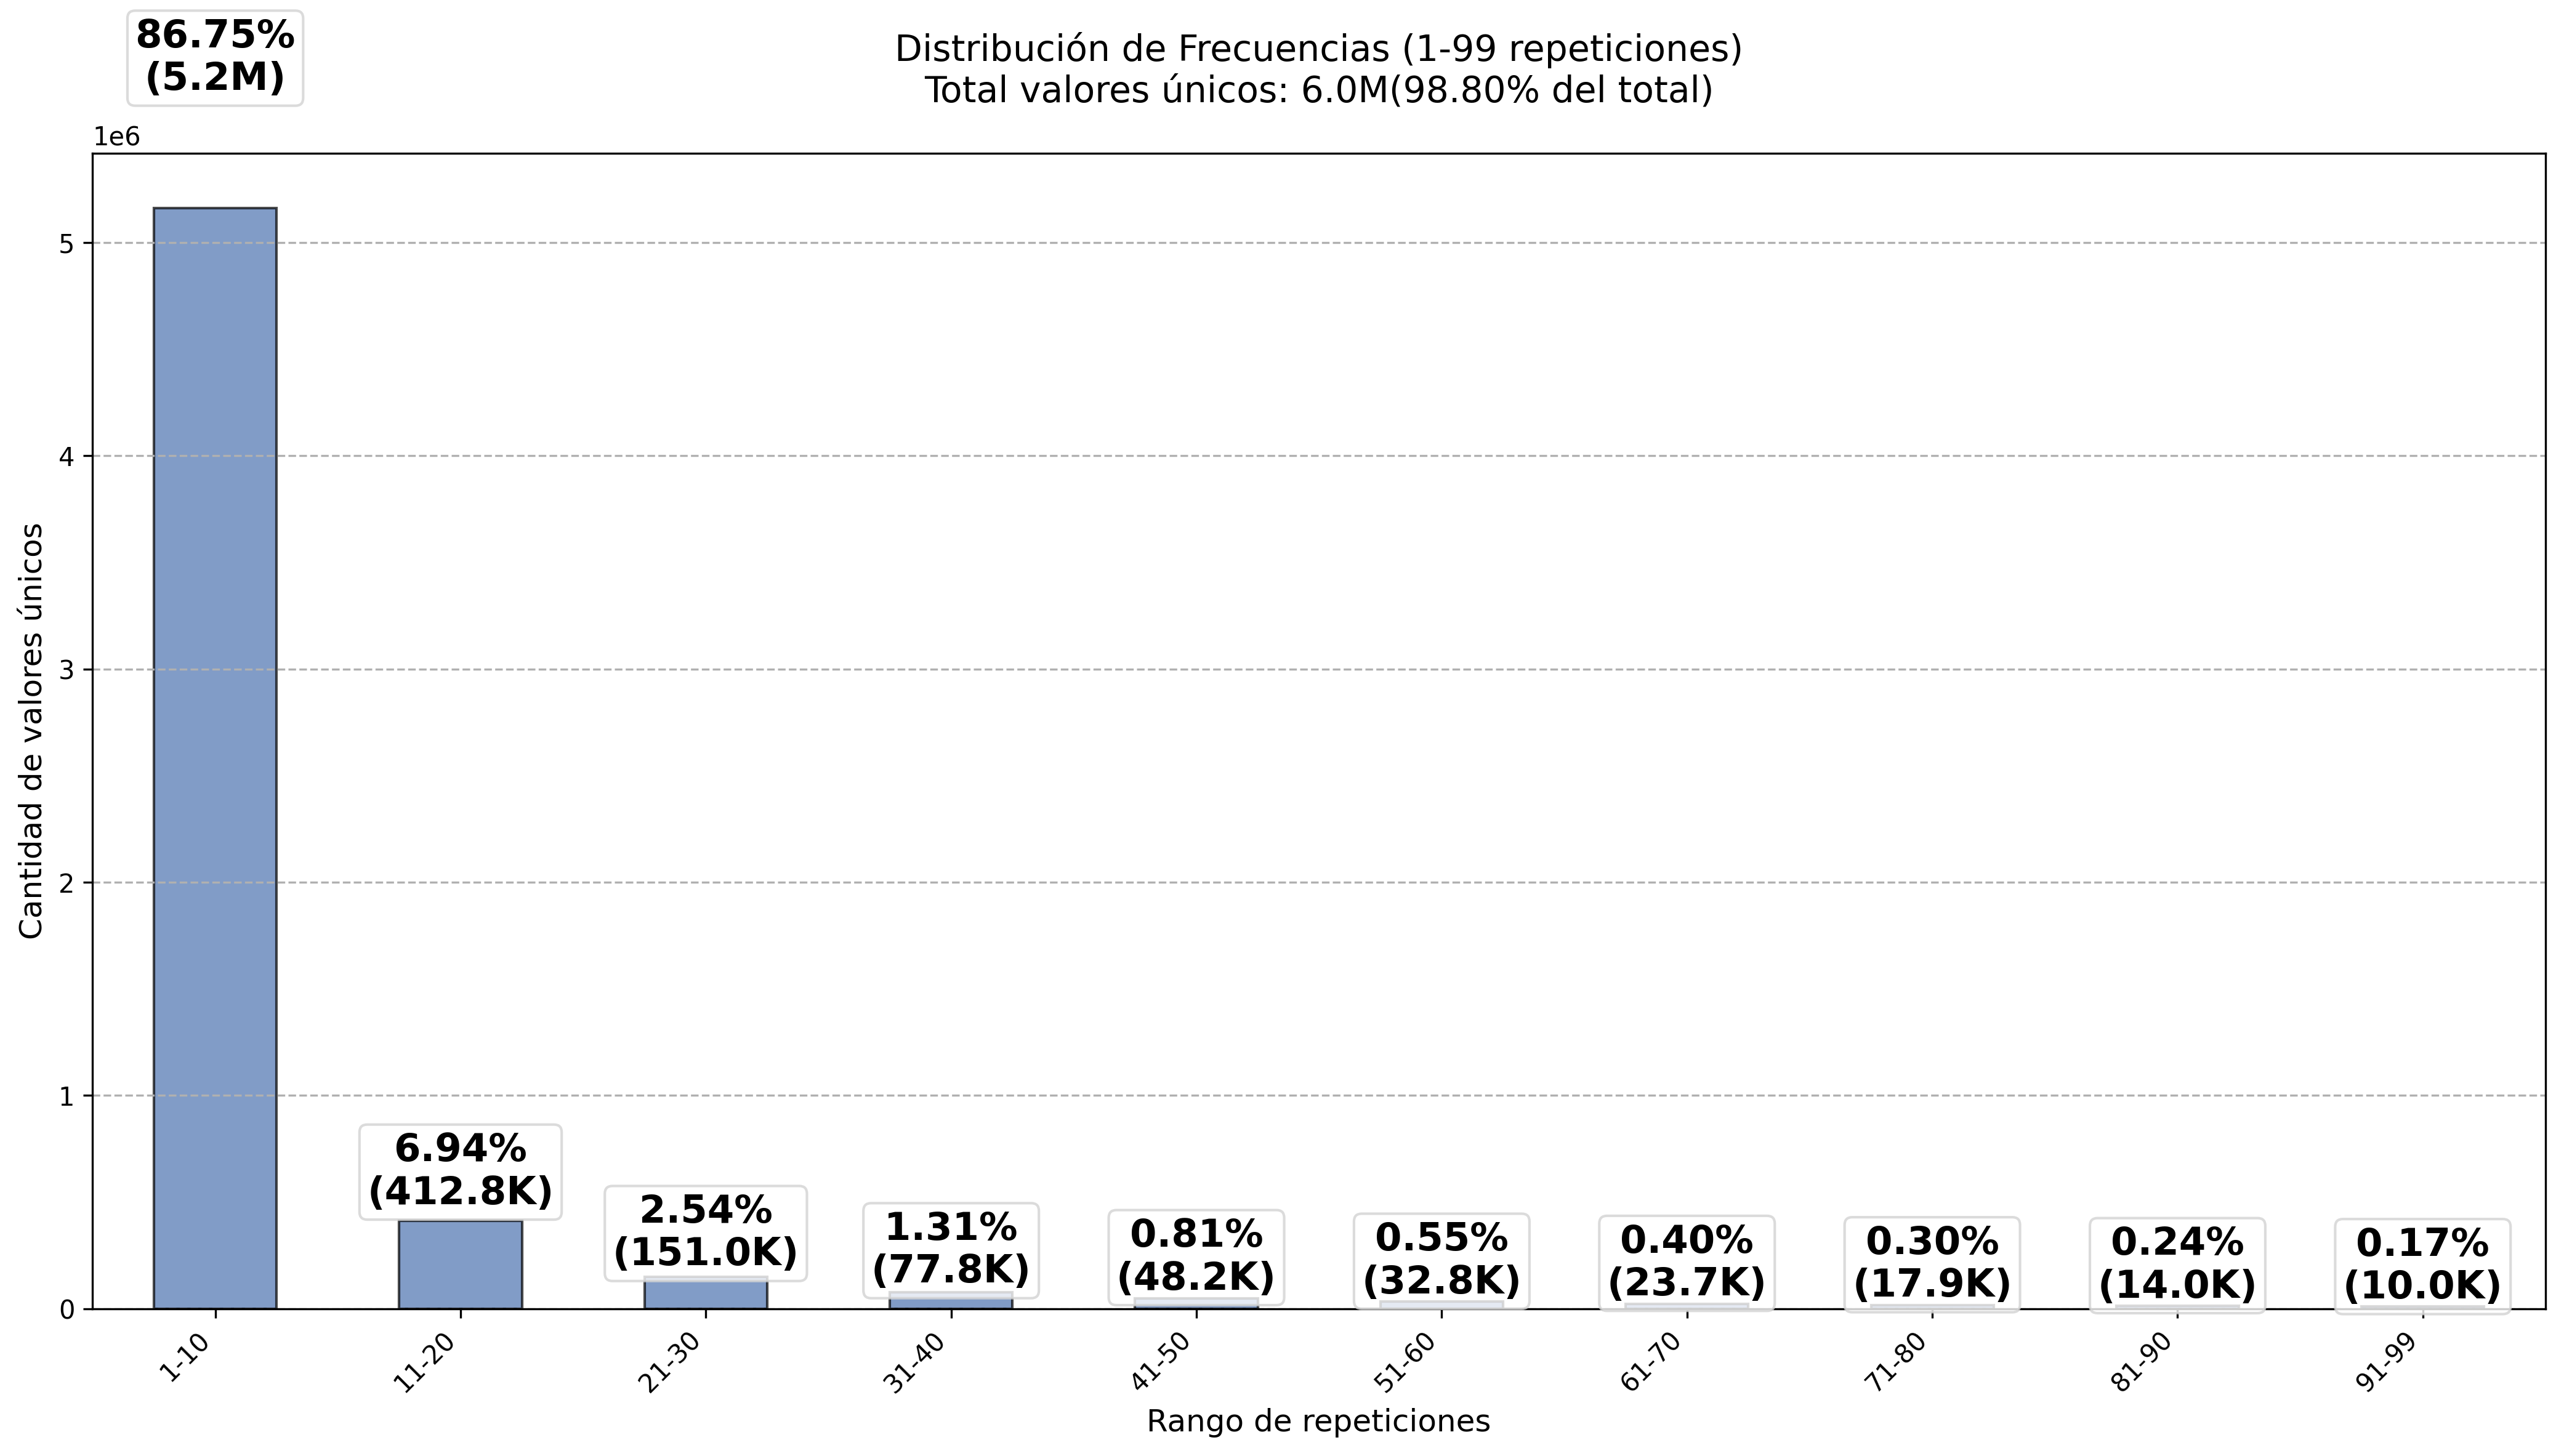
\includegraphics[width=\linewidth]{img/histograma_1-99_identifier_Mobility_Data_Slim_DeDuplicate.png}
        \caption{Histograma 1-99 repeticiones}
        \label{fig:sub1}
    \end{subfigure}
    \hfill
    \begin{subfigure}[t]{0.48\textwidth-1em}
        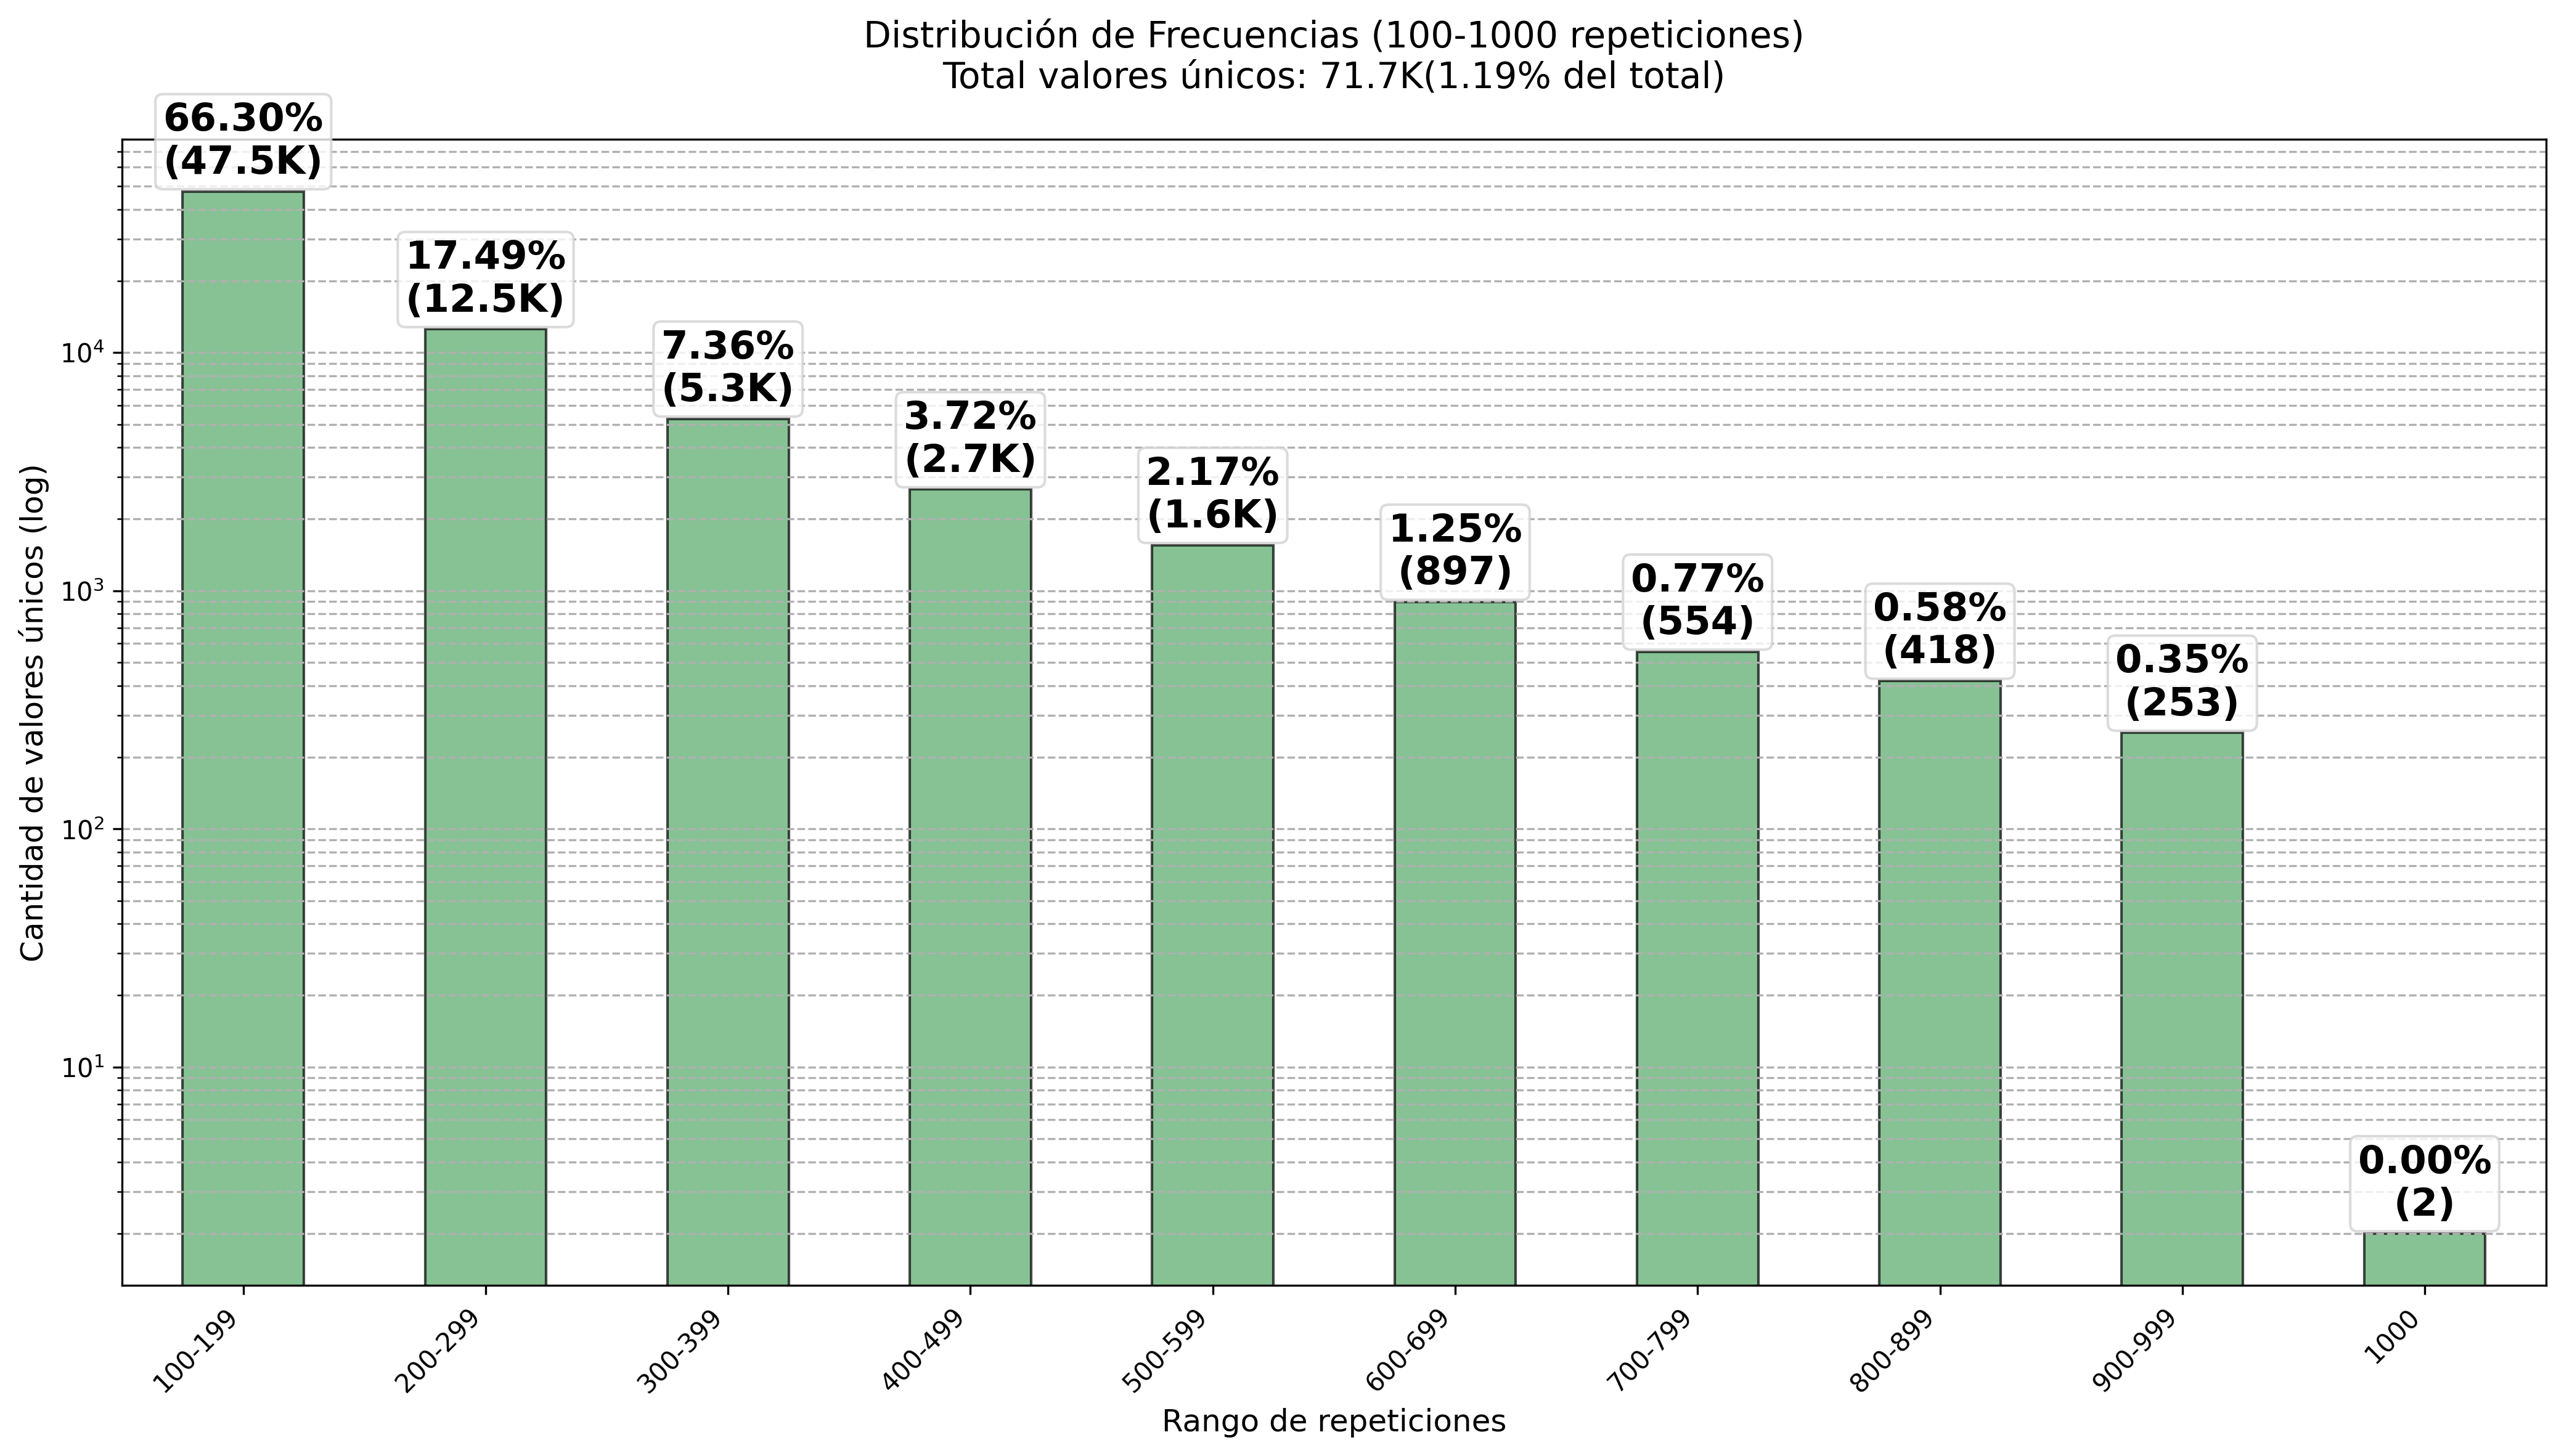
\includegraphics[width=\linewidth]{img/histograma_100-1k_identifier_Mobility_Data_Slim_DeDuplicate.png}
        \caption{Histograma 100–1000 repeticiones}
        \label{fig:sub2}
    \end{subfigure}

    \vspace{0.5cm}

    \begin{subfigure}[t]{0.48\textwidth}
        \centering
        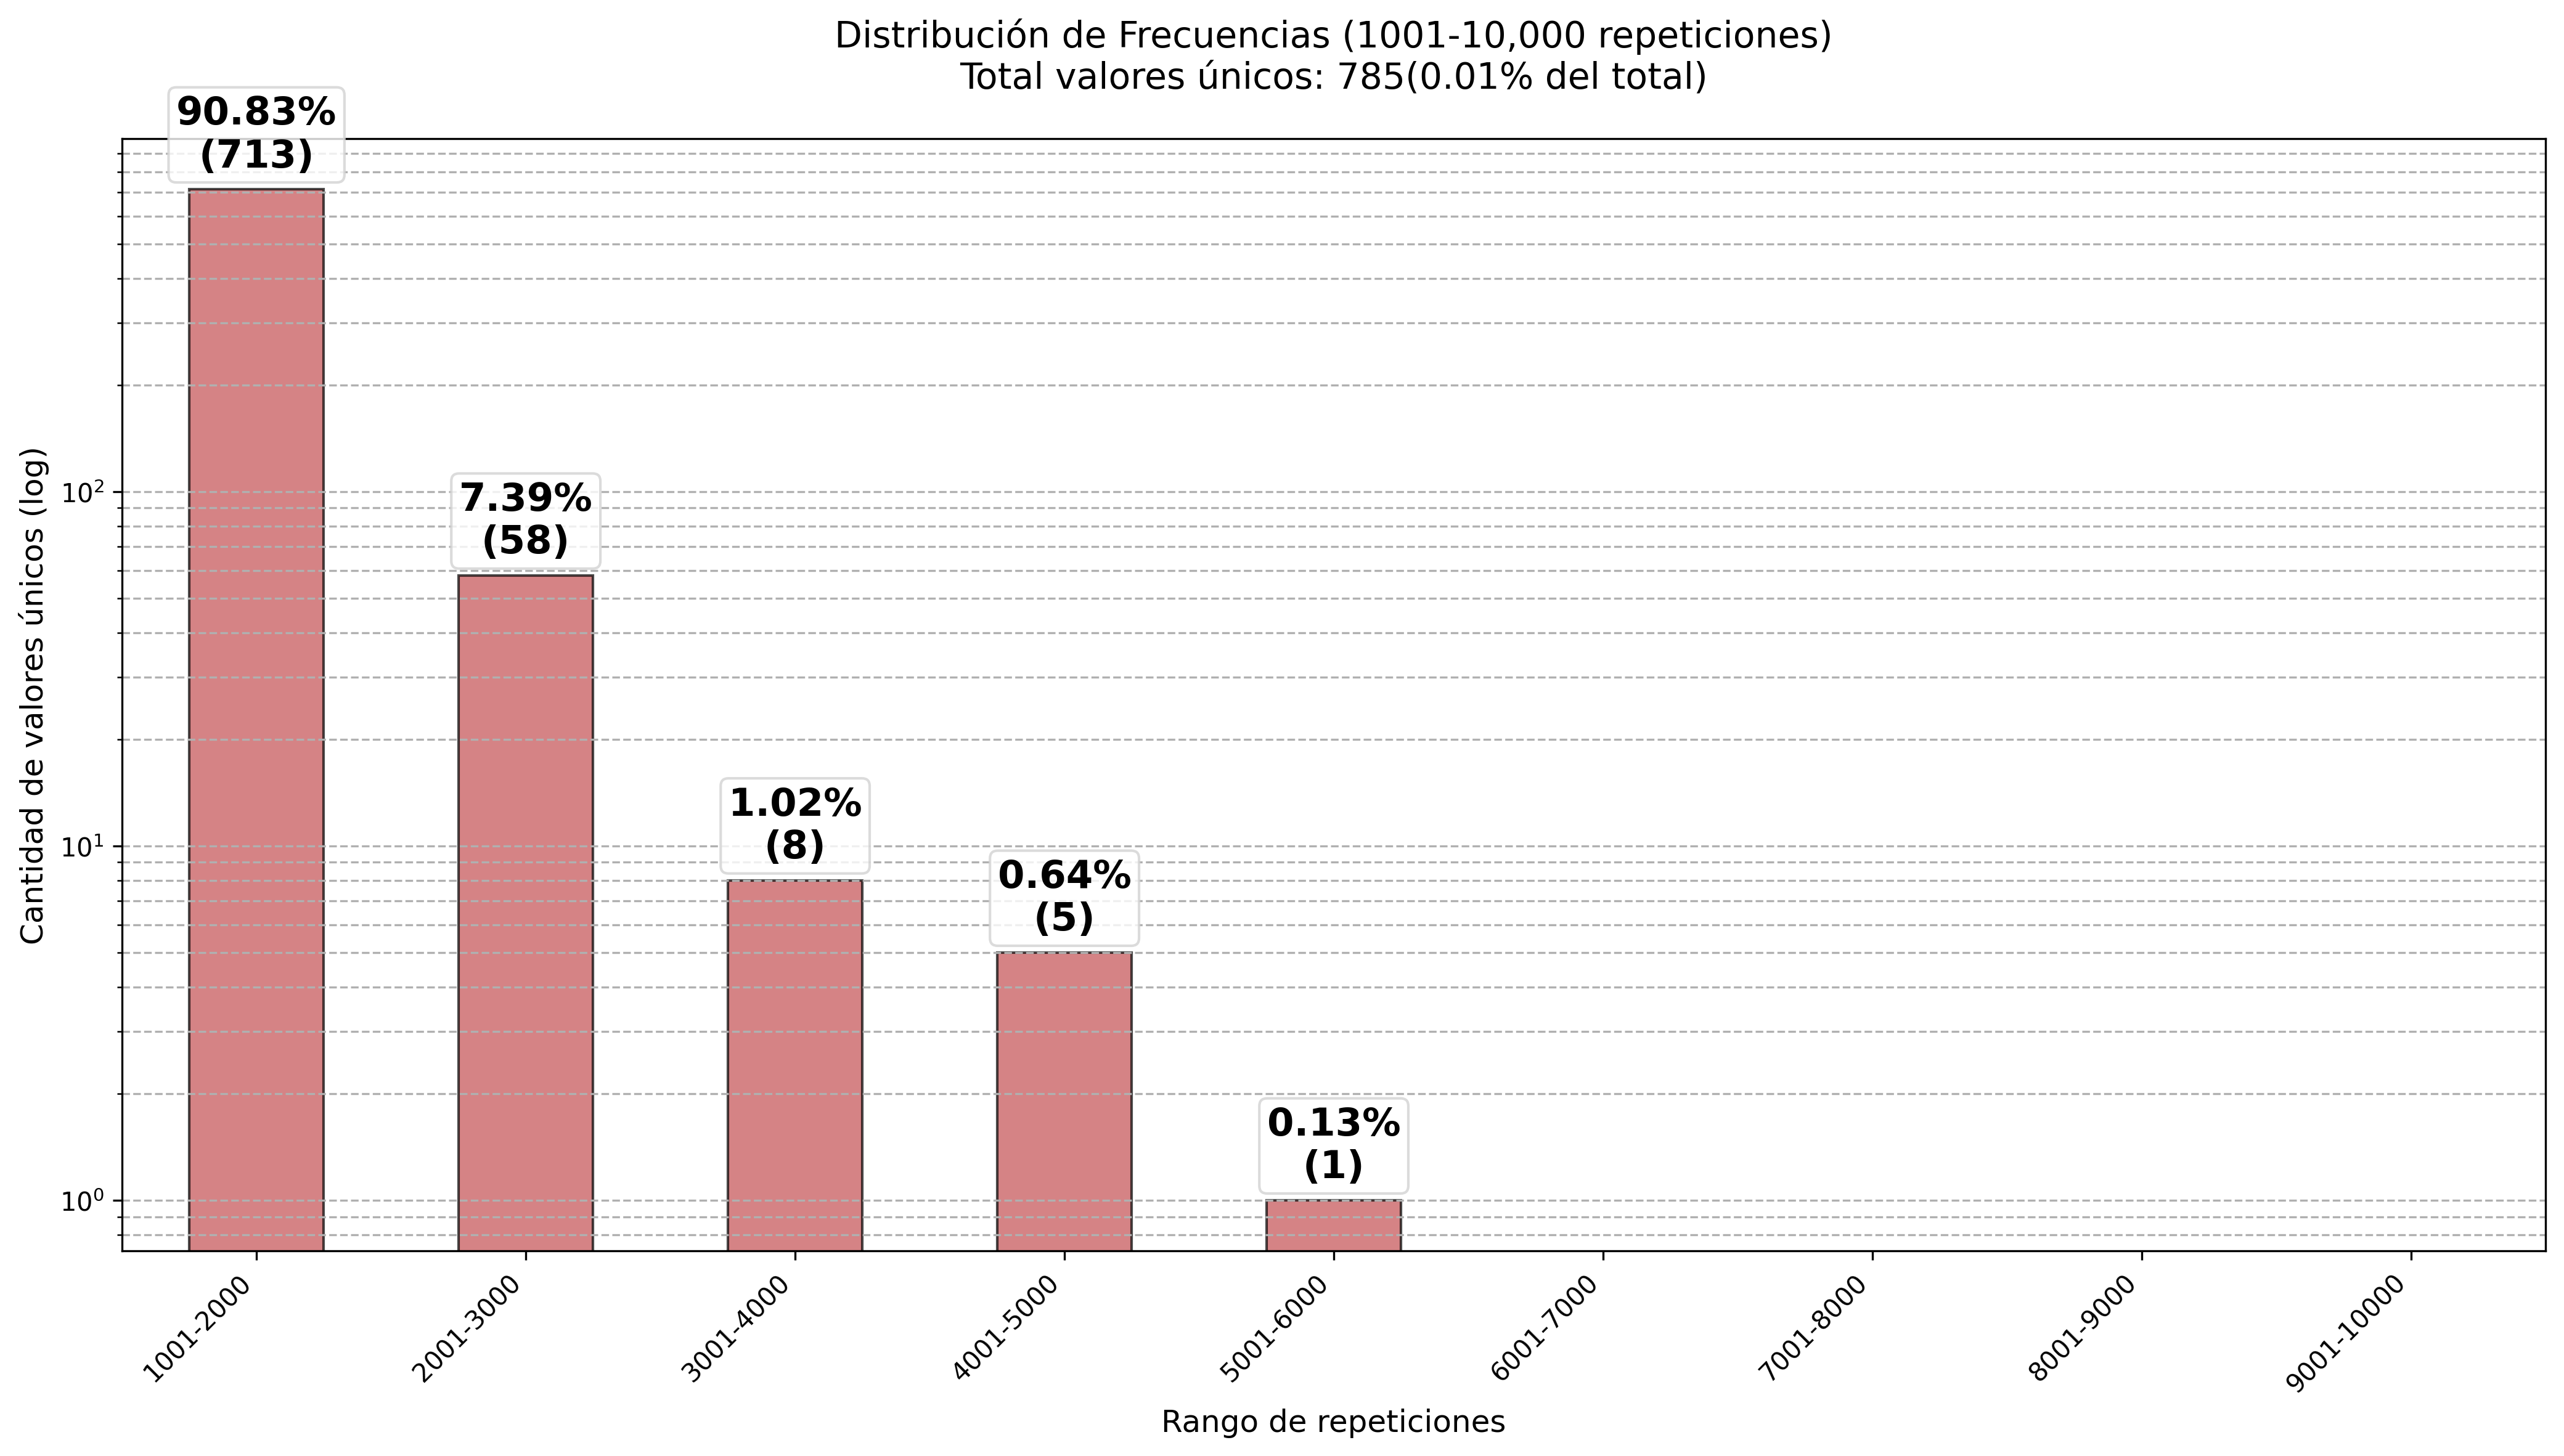
\includegraphics[width=\linewidth]{img/histograma_1k-10k_identifier_Mobility_Data_Slim_DeDuplicate.png}
        \caption{Histograma 1001–10000 repeticiones}
        \label{fig:sub3}
    \end{subfigure}

    \caption{Comparación de histogramas por rangos de repeticiones.}
    \label{fig:histogramasDeDuplicate}
\end{figure}
\end{document}

